\chapter{Concepts of a Cache-Aware Measurement System}\label{ch:measurement}

% [SKELETON] cache-aware focus. The task assignment is made SELF-EXPLANATORY here (nobody reads it)
% and draws on ALL concerns of Chapter 2. ALL tables live in this chapter.

Building on the foundations from Chapter~\ref{ch:foundations}, this chapter first develops the problem
statement and the requirements for a measurement system, and as their \emph{solution} the anatomy model
and the measurement system built upon it --- demonstrated on the probe PRT-ART\@. In doing so, the
chapter newly introduces three orderings that Chapters~\ref{ch:impl} to~\ref{ch:conclusion} presuppose:
the triad of the axes into measurement, system, and organ axes, the four carrier stages of the
apparatus --- planner, CacheEngineBuilder, tier binary, and hybrid tier binary --- with their identity
stamp, and the store in which what is built and what is measured lies under stamp keys.

\section{Problem Statement and Requirements for a Measurement System}\label{sec:task-concerns}
The starting point is the finding of the foundations (Chapter~\ref{ch:foundations}): the performance of
cache-aware search structures is decided not by asymptotic complexity but by cache-line behaviour under
real load. This behaviour, however, is the result of many interlocking design decisions --- how nodes
branch, how pages are arranged in memory, how allocation, prefetching, and synchronization are done ---,
and in the published methods these decisions have grown together monolithically: whoever measures a
method always measures the whole bundle, never the individual decision. Precisely this is the problem
statement of this thesis, the \emph{separability problem}: the contribution of each individual design
decision to cache-line behaviour shall become visible in isolation --- per decision as well as for the
whole algorithm.

The state of the art sharpens this problem in two directions. In substance, each of the studied works
optimizes only a few design decisions in isolation, and in the studied corpus \emph{not a single method
occupies all design dimensions together}: some dimensions are filled exclusively with baseline or
textbook variants (the mapping between algorithm and cache traversal), others appear only as a
\emph{measurement target} (the dTLB), the spatial search class is missing entirely, and decisions such as
I/O, migration, filtering, and buffering are each occupied individually but never together with the
search decisions in one design. Methodologically a second gap is added: results are reported in
incomparable settings, and the frequent choice of scenario-specific, often favourably tailored load
profiles hampers a fair cross-comparison; what is missing is a bias-reduced measurement of \emph{all}
load profiles against \emph{all} methods on a common basis.

From this double gap follow four requirements for a solution. It must, first, \emph{decompose}
cache-aware search algorithms into interchangeable design constituents, so that each decision becomes
individually graspable; second, \emph{reconstruct} the state-of-the-art designs as explicit
configurations of these constituents, so that the known and the new become comparable in the same space;
third, \emph{measure} the cache-line-aware behaviour per constituent as well as for the whole algorithm
on a common basis --- all load profiles against all methods, bias-reduced; and fourth, derive the best
overall algorithm from the measurements and \emph{deliver} it system-optimized --- realized as a ranking
per interface function and metric, as a Pareto front of non-dominated candidates, and as a delivery
artefact of binary, version sidecar, and manifest (Section~\ref{sec:heuristics-loop}). The cache-aware
focus is no side condition but the guiding quantity: precisely the cache-line behaviour that decides
performance shall become measurable in isolation per design decision.

The measurement requirement sharpens, at the juxtaposition of cache-aware and cache-oblivious designs
(Section~\ref{sec:hardware-history}), into a third, intermediate path: the actual cache properties (line
size, hierarchy depth, topology) are \emph{determined} per target platform and enter a system-optimized
binary as fixed quantities, while the \emph{configurable} cache-near settings are permuted as sub-axis
parameters against an already-loaded binary --- in the measurement realm these are the registered
dynamic dimensions prefetch distance, pool budget, batch size, inline threshold, thread count, and
workload as well as, where architecture and operating system permit, the hardware prefetcher, graded by
what hardware and operating system allow, from fully runtime-configurable (mutable Linux with MSR access)
through boot- or compile-static (immutable operating systems) to fixed (read-only cache registers on ARM
and RISC-V); which grade a platform offers is determined by the planner's platform probe. Thus
cache-oblivious behaviour is augmented with \emph{measured} locality knowledge.

The four requirements condense into a target picture, the \emph{design space}: each partial decision ---
say node type, memory layout, or allocator --- spans an axis of its own, and every state-of-the-art
algorithm is a point in the Cartesian product of these axes (Figure~\ref{fig:design-space}).
\begin{figure}[htbp]\centering
\begin{tikzpicture}[font=\footnotesize,>=Stealth,thick]
  \draw[->] (0,0) -- (4.8,0) node[right,font=\scriptsize,align=left]{node\\type (T4)};
  \draw[->] (0,0) -- (0,3.3) node[above,font=\scriptsize]{layout (T5)};
  \draw[->] (0,0) -- (-1.7,-1.3) node[below left,font=\scriptsize]{allocator (T6)};
  \foreach \x in {1,2,3}\foreach \y in {1,2,3}{\fill[black!35] (\x,\y) circle (1.6pt);}
  \fill[red] (2,2) circle (3.2pt);
  \node[red,right] at (2.15,2.25){ART $=$ one point};
  \node[draw,rounded corners,fill=blue!5,align=left,font=\scriptsize] at (3.5,2.95){\textbf{Legend:} 3 of\\18 organ axes (T0--T17)};
  \node[align=center,font=\scriptsize] at (1.6,-2.2){Every state-of-the-art algorithm\\$=$ one point in the Cartesian product of the axes};
\end{tikzpicture}
\caption{The design space: the axes span a multidimensional Cartesian product; a concrete algorithm is a point within it. For illustration, three of the eighteen organ axes are chosen --- the real storage organ of node type~(T4), memory layout~(T5) and allocator~(T6); the full design space has eighteen organ dimensions; to these is added an optional nineteenth organ axis for disk I/O, which does not describe an assignment but describes how other axes are described (Section~\ref{sec:axis-triad}).}\label{fig:design-space}
\end{figure}

Once the design space is spanned this way, the separability problem becomes solvable: varying a design
decision means moving along exactly one axis while all others stay fixed --- its contribution becomes
measurable in isolation. What this thesis contributes is consequently the systematic, orthogonal axis
decomposition of the known designs together with a \emph{permuted measurement architecture} that
reconstructs them as explicit configurations and measures them on a common basis; for cache-aware
algorithms cannot be differentiated without a separation of the properties that decisively govern
caching. The four requirements at the same time describe a processing chain --- from the definition of an
axis assignment through its generation and measurement to the evaluation ---, and a system of this size
remains manageable only if these stations are developed as separate layers with fixed contracts; the
layer model for this is developed in Section~\ref{sec:anatomy-layers}. Which of the catalogued instances
the framework adopts and which it replaces as obsolete is developed dialectically by the following
Section~\ref{sec:sota-instances}; the solution concept
(Section~\ref{sec:anatomy-model}) and the measurement system built upon it
(Section~\ref{sec:measurement-system}) are the solution that closes the double gap.

\section{State of the Art as Axis Instances}\label{sec:sota-instances}
The methods known from Chapter~\ref{ch:foundations} now appear systematically as axis compositions;
the complete catalogues of this dissection are gathered in the present section.
This adoption proceeds \emph{dialectically} (thesis--antithesis--synthesis): per axis a foreign organ is
\emph{adopted} (thesis) or an obsolete assumption is \emph{replaced} (antithesis), from which the own
contribution emerges as synthesis. The guiding idea is the \enquote{third way} from
Section~\ref{sec:task-concerns} --- measured locality knowledge instead of hard-wired or ignored cache
awareness ---, which makes each axis explicit as an orthogonal, permutable, and individually measurable
organ. For many axes the antithesis is not an obsolete foreign instance but the implicit assumption of not
regarding the decision as selectable at all; the synthesis then consists in making it an explicit axis in
the first place (marked \enquote{---} in the replaced column). Two cluster assignments are deliberate
approximations: the cache-traversal axis~(T1) draws its inspiration from the layout theory as well as
from prefetching, and the reclamation sub-axis of the allocator~(T6) shares its sources with the
synchronization~(T8) --- an inter-organ wiring, not a cluster violation. The dialectical comparison is
carried by the living-being metaphor: every catalogued method is a living being whose organ --- the
assignment of an axis --- is adopted or replaced, and the framework is the living being that arises from
the adopted organs. The metaphor itself (organ, blood, habitat, laboratory) is defined in
Section~\ref{sec:anatomy-metaphor}; here it is only touched upon.
Table~\ref{tab:dialectic} summarizes this adoption per composition axis.

{\footnotesize
\begin{longtable}{@{}p{2.3cm}p{3.7cm}p{2.7cm}p{3.6cm}@{}}
\caption{Dialectical adoption of the state-of-the-art instances per composition axis (in canonical slot order T0--T17; telemetry and target ISA belong to the system sphere and to the measurement tooling, respectively, Section~\ref{sec:axis-triad}. Cluster codes: A~trie/node, B~hybrid/layout, C~allocation, D~prefetching, E~synchronization, F~hardware/measurement/engineering)}\label{tab:dialectic}\\
\toprule
\textbf{Axis} & \textbf{adopted (thesis)} & \textbf{replaced (antithesis)} & \textbf{synthesis core} \\
\midrule
\endfirsthead%
\toprule
\textbf{Axis} & \textbf{adopted} & \textbf{replaced} & \textbf{synthesis core} \\
\midrule
\endhead%
\bottomrule
\endlastfoot%
T0 Search-Algorithm (A) & ART, HOT, START, SuRF, Wormhole; k-ary/interpolation search & monolith \enquote{structure is method} & search paradigm as a permutable axis \\
T1 Cache-Traversal (B) & cache-line stride (Chen), cache-oblivious (Bender), HBM (Schmidt) & implicit textbook linear search & algorithm and cache view separated \\
T2 Mapping (B) & linear 1:1 mapping; hash redirect, permutation index & --- & direct vs.\ pool-relative mapping made explicit \\
T3 Path-Compression (A) & byte-wise (ART), Patricia (HOT), macro node (CoCo), multi-byte (START) & uncompressed raw path & compression granularity selectable \\
T4 Node-Type (A) & ART Node4/16/48/256 & fixed node size & adaptive node class + storage delegation \\
T5 Memory-Layout (B) & AoS-aligned, SoA, LOUDS bit-packed, CSS/CSB\textsuperscript{+}, AoSoA & --- & four layout dimensions permutable \\
T6 Allocator (C) & A01--A23 (Hoard, mimalloc, jemalloc, TCMalloc, \ldots) + RCU/Hazard & algorithm-hardwired allocator & allocation as shared interface organ (seven sub-axes) \\
T7 Prefetch (D) & distance estimator (ART), hardware (Wormhole), stride (Chen), adaptive & prefetch not isolated as an axis & path-oriented bundle prefetch (own) \\
T8 Concurrency (E) & OLC (ART), RCU, hazard pointers; lock-/wait-free & coarse locking as the only assumption & pattern $\perp$ reclamation as two sub-axes \\
T9 Serialization (F) & raw binary, varint (ART), succinct (LOUDS/FST), LZ77 & --- & encoding/compression selectable \\
T10 Value-Handle (F) & inline, external pool, immutable shared (RCU), versioned & implicitly fixed embedded value & placement, ownership and versioning (+ chain ref) \\
T11 Index-Organization (B) & clustered, IOT, non-clustered, heap & --- & storage order as its own axis \\
T12 I/O-Dispatch (F) & buffered, mmap, direct I/O & mmap as anti-pattern & persistence decoupled from the search structure \\
T13 Migration (F) & hot/cold, multi-tier NVM, LeCaR-ML & tiering never combined with search axes & migration logic as a measurable axis \\
T14 Filter (F) & Bloom, Cuckoo, SuRF-range, Xor & filter never integrated with search axes & filter as an orthogonal organ \\
T15 Queuing-q1 (F) & Disruptor ring, delta chain, CoW, epoch-RCU, SPSC/MPMC & operations buffer never an axis & buffer with access-pattern classes \\
T16 Queuing-q2 (F) & eager/lazy, watermark (LSM), timed & flush policy implicit & adaptive EWMA flush policy (own) \\
T17 Persistence-Target (F) & in-memory storage as the standard target & implicit in-memory assumption & persistence target as its own axis (pinned to in-memory in the measurement catalogue) \\
\midrule
\multicolumn{4}{@{}l}{\emph{Quantities of the system and measurement sphere (Section~\ref{sec:axis-triad}):}} \\
target\_isa (system) & vendor-spec x86-64/AArch64/Power/RISC-V (+ SIMD) & --- & target ISA as a system complex axis \\
Telemetry (system/meas.) & density tracker, insert counter, HdrHistogram, path counter & per-node counter
  (cache-line ping-pong) & coherence-friendly leaf-only; split in two: measurement sub-axis $+$ build quantity \\
\end{longtable}
}

The systematic core is the axis-wise \emph{dissection}: every overall algorithm is decomposed into its
organs, and per axis the contributing organ algorithms are listed, with a brief reference to the
originating living being. The framework carries \emph{eighteen organ composition axes} in fixed
slot order (T0--T17); alongside them stand the quantities of the system sphere --- target ISA,
SIMD and extension hardware as well as the two-way-split telemetry (the triad of axis categories
is ordered by Section~\ref{sec:axis-triad}) --- and the probe build axis page type. Besides the eighteen
canonical organ main axes --- a \emph{main axis} is an axis whose chosen assignment is compiled
compile-statically into the binary --- the organ catalogue carries an optional
\emph{organ meta-meta axis} for disk I/O (\emph{meta-meta} means: the axis does not describe an
assignment but describes how other axes are described; the short definition together with the ordering
of levels is given in Section~\ref{sec:axis-triad}), which takes effect only with a disk-writeback
target and is built in compile-statically. Many axes are refined into \emph{sub-axes} --- axes beneath a
main axis: as static sub-axes a compile-time choice among partial algorithms (say SA1--SA4 or AA1--AA7),
as dynamic sub-axes runtime parameters that are varied without recompilation --- and provide other axes
with distributed interfaces for their detail operations --- exactly these \emph{axis interfaces} are
captured by the micro-benchmarking (Section~\ref{sec:mess-chain}), which collects runtime and success
parameters per interface call (Section~\ref{sec:measurement-system}).
Table~\ref{tab:axes-overview} gives the overview of which publications contribute an organ per
axis; the thematic origin clusters of the prior works thereby appear \emph{dissolved} into their organ
contributions.

\begin{table}[!htbp]
  \caption{Axis dissection of the search methods: eighteen organ axes in canonical
  slot order (T0--T17), the quantities of the system and measurement sphere, the
  probe build axis, and the optional organ meta-meta axis; per axis the sources contributing an organ.}\label{tab:axes-overview}
  \centering\footnotesize
  \begin{tabular}{@{}l l p{6.8cm}@{}}
    \toprule
    \textbf{Axis} & \textbf{Sub-axes} & \textbf{Contributing sources} \\
    \midrule
    T0 search\_algo & SA1--SA4 & P01,P02,P05,P07,P10; k-ary (TUD 2009), interpol., Eytzinger, skip list, B-tree, hash \\
    T1 cache\_traversal & CT1--CT2 & cache-line default; P17,P21,P32 \\
    T2 mapping & MP1--MP2 & P03,P07; CE baseline \\
    T3 path\_compression & PC1--PC3 & P01,P02,P04,P05,P09 \\
    T4 node\_type & NT1--NT3 & P01,P02,P03,P04,P05,P06,P11,P12,P13 \\
    T5 memory\_layout & HM1--HM3\textsuperscript{b} & P06,P09,P11,P12,P32; default \\
    T6 allocator\textsuperscript{a} & AA1--AA7 & A01--A23; P29,P30 \\
    T7 prefetch & PF1--PF3 & P07,P21,P23,P25,P26,P27 \\
    T8 concurrency & CC1--CC2 & P08,P29,P30; Dijkstra,Courtois,Herlihy,Michael/Scott \\
    T9 serialization & SR1--SR3 & P01,P09,P10; LZ77 \\
    \midrule
    T10 value\_handle & VH1--VH3 & P01,P03,P07,P29 \\
    T11 index\_organization & io1--io3 & Bayer/McCreight,Comer,Oracle \\
    T12 io\_dispatch & IO1--IO3 & Stonebraker,Crotty; baselines \\
    T13 migration\_policy & MG1--MG3 & anti-caching,NVM-tiering,LeCaR\@; none \\
    T14 filter & FT1--FT3 & Bloom,Cuckoo,P10,Xor \\
    T15 queuing\_q1 & QS1--QS6 & Disruptor, Bw-tree, Driscoll, P29, Pugh, LSM, Lamport, Michael/Scott \\
    T16 queuing\_q2 & FS1--FS4 & eager/lazy/watermark/Kafka/RocksDB \\
    T17 persistence\_target & --- & CE baseline (in-memory); disk writeback as a disabled option \\
    \midrule
    Sys.\ target\_isa & IS1--IS3 & x86-64/AArch64/Power/RISC-V (vendor-spec) \\
    Sys.\ external\_utils: SIMD & SE1--SE3 & SSE2/AVX2/AVX-512/NEON/SVE2/RVV\@; GPU\@: CUDA \\
    Sys.\ external\_utils: ext.\ HW & HW1--HW4 & HW strategy per publication (Tab.~\ref{tab:hw-sched}) \\
    Sys./meas.\ telemetry & TM1--TM3 & P01,P02,P16,P17,P26,P28; HdrHistogram (Gil Tene) \\
    Build (probe) page\_type & PG1--PG3 & P01,P02,P04,P05,P06,P10,P11,P12,P13,P20; PRT-ART (2026) \\
    Organ meta-meta disk\_io & staging (runtime) & CE baseline; optional, disabled (Section~\ref{sec:axis-triad}) \\
    \bottomrule
  \end{tabular}

  \smallskip
  {\footnotesize \textsuperscript{a}~Corpus of 23 works (A01--A23); the code provides 26 vendor implementations.\par}
  {\footnotesize \textsuperscript{b}~HM4 (stride pattern) is a planned fourth sub-axis without a carrying layout building block; the code carries no tag for it (Appendix~\ref{app:blocks}, Section \enquote{T5 Memory Layout}).\par}
\end{table}

The \emph{search axis} (T0) comprises the most organs --- as original bindings ART~\cite{leis2013art},
HOT~\cite{binna2018hot}, START~\cite{fent2020start}, SuRF~\cite{zhang2018surf}, and
Wormhole~\cite{wu2019wormhole}, plus generic search methods such as k-ary search~\cite{schlegel2009kary},
interpolation search~\cite{perl1978interpolation}, Eytzinger-layout search~\cite{khuong2017eytzinger},
skip list~\cite{pugh1990skiplist}, B-tree~\cite{bayer1972btree}, and
open-addressing hashing~\cite{knuth1998taocp3}. The traversal axes separate the
algorithm and cache views: in the code T1 contains the three traversal building blocks
\texttt{Linear\allowbreak{}Fanout}, \texttt{Hash\allowbreak{}Lookup}, and
\texttt{Binary\allowbreak{}Search\allowbreak{}Fanout}; the related literature spans the axis from
cache-line walking through stride prefetch~\cite{chen2001prefetch} and HBM proximity~\cite{schmidt2025hbm} to
cache-oblivious recursion~\cite{frigo1999cache} (Appendix~\ref{app:blocks}), while T2 (mapping)
remains a sparsely occupied axis with the linear 1:1 mapping (\texttt{Direct\allowbreak{}Placement}) and the
pool-relative offset mapping (\texttt{Pool\allowbreak{}Relative}) --- hash
redirect~\cite{wu2019wormhole} (MP04) and permutation index~\cite{mao2012masstree} (MP03) are carried
by the code as roadmap values without a registry entry. The \emph{path compression} (T3)
instantiates the byte-wise variant~\cite{leis2013art}, the Patricia split~\cite{morrison1968patricia,binna2018hot},
and the pass-through variant \texttt{None}; the macro node~\cite{boffa2024coco} and the
multi-byte rewiring~\cite{fent2020start} are related literature of the axis without a building block of
their own (the sub-axis PC1 carries the granularity \texttt{multi-byte} as a tag), and the
\emph{node-type axis} (T4) bundles in the code the four adaptive ART node formats
Node4/16/48/256~\cite{leis2013art}; HOT compound~\cite{binna2018hot}, Internal/Border~\cite{mao2012masstree},
Decision/Span~\cite{schmeisser2022b2tree}, LOUDS-Dense/Sparse~\cite{zhang2018surf}, and the
CSS/CSB\textsuperscript{+}/Hankins nodes are paper node formats (reconstruction targets of this
thesis, not a CE baseline); the PRT-ART profile family is brought in by the probe via its build axis page type.

The \emph{memory-layout axis} (T5) ranges in the code from the cache-line-aligned AoS
(\texttt{AoS\allowbreak{}Strict\allowbreak{}Memory\allowbreak{}Layout},
\texttt{Cache\allowbreak{}Line\allowbreak{}Aligned\allowbreak{}Memory\allowbreak{}Layout}) through SoA and AoSoA to the
bit-packed LOUDS layout
(\texttt{Packed\allowbreak{}Bitmap\allowbreak{}Memory\allowbreak{}Layout})~\cite{jacobson1989louds}; pointer-free
arrangement~\cite{rao1999css}, sibling cluster~\cite{rao2000csb}, and embedded
tree~\cite{schmeisser2022b2tree} are related literature of the axis (Appendix~\ref{app:blocks}). The
\emph{allocator axis} (T6) is the most densely occupied with the corpus A01--A23 and is refined into seven
sub-axes --- from free-list topology through thread locality/NUMA affinity~\cite{ungethuem2017survey}
and the allocation strategy to reclamation (epoch, RCU~\cite{mckenney2001rcu},
hazard pointers~\cite{michael2004hazard}, QSBR); the code provides 26 allocator implementations for the
23-work corpus (individual works contribute several variants); the 23 allocator profiles with licence
and workload affinity are listed by Table~\ref{tab:allocator-profiles}, ten of them attached with
adapter and original code. The \emph{value axis} (T10) distinguishes inline value~\cite{leis2013art}, external
pool~\cite{wu2019wormhole}, versioned pointer~\cite{mao2012masstree}, immutable
shared ref~\cite{mckenney2001rcu}, and the chained external reference (ChainRef, a local re-implementation
without a paper template) --- five of five building blocks of the registry ---, the \emph{serialization axis} (T9)
raw binary, succinct LOUDS/FST, and
varint~\cite{leis2013art}.

\begin{table}[!htbp]
  \caption{Allocator profiles (23, all with \texttt{expected\_workload} tag) with licence, workload affinity, and attachment state}\label{tab:allocator-profiles}
  \centering\small
  \begin{tabular}{lllll}
    \toprule
    \textbf{Profile} & \textbf{Family} & \textbf{Licence} & \textbf{expected\_workload} & \textbf{Code} \\
    \midrule
    hoard & A01 & Apache-2.0 & YCSB\_A & yes \\
    slab & A02 & none & YCSB\_A & --- \\
    michael\_lockfree & A03 & LGPL-2.1-or-later & YCSB\_B & yes \\
    mimalloc & A04 & MIT & YCSB\_A & yes \\
    jemalloc & A05 & BSD-2 & YCSB\_B & yes \\
    tcmalloc & A06 & Apache-2.0 & YCSB\_C & yes \\
    snmalloc & A07 & MIT & YCSB\_A & yes \\
    scalloc & A08 & BSD-3 & YCSB\_A & yes \\
    numalloc & A09 & unknown & YCSB\_B & --- \\
    rpmalloc & A10 & Public Domain & YCSB\_C & yes \\
    lrmalloc & A11 & MIT & YCSB\_B & yes \\
    cama & A12 & none & YCSB\_A & --- \\
    starmalloc & A13 & Apache-2.0 & YCSB\_B & --- \\
    tcmalloc\_warehouse & A14 & Apache-2.0 & YCSB\_C & --- \\
    hmalloc & A15 & none & YCSB\_B & --- \\
    pim\_malloc & A16 & MIT & YCSB\_E & --- \\
    crystalline & A17 & unknown & YCSB\_B & --- \\
    exgen\_malloc & A18 & unknown & YCSB\_C & --- \\
    buddy & A19 & none & YCSB\_C & --- \\
    dlmalloc & A20 & Public Domain (CC0) & YCSB\_C & yes \\
    ptmalloc2 & A21 & LGPL-2.1+ & YCSB\_B & --- \\
    pmr\_resource & A22 & Standard-Library & YCSB\_B & --- \\
    vmem\_magazines & A23 & none & YCSB\_A & --- \\
    \bottomrule
  \end{tabular}

  \smallskip
  {\footnotesize \texttt{expected\_workload} = YCSB workload class (A/B/C/E); licence verbatim from the profile
  (none = no OSS code, unknown = not recorded in the profile); Code = adapter and original code present in the
  repository (yes) or documentation dossier without adapter (---). Two reference quantities: 23 profiles A01--A23
  (profile count of this table) versus 26 allocator wrappers of the code (wrapper count,
  Appendix~\ref{app:blocks}): there A22 splits into the three standard-library baselines A22a--A22c
  (\texttt{std\_malloc}, \texttt{pmr\_resource}, \texttt{pool\_resource}), and the allocator front A24
  reconstructed from the SOTA profile P33 joins without an allocator profile of its own.\par}
\end{table}

On the hardware-near side, the \emph{prefetch axis} (T7) contains four building blocks in the code --- no
prefetch (\texttt{None\allowbreak{}Prefetch}, measurement baseline), the distance-estimated software prefetch after
ART~\cite{leis2013art} (\texttt{Distance\allowbreak{}Estimator\allowbreak{}Prefetch}), the explicit
hardware prefetch instruction from Wormhole~\cite{wu2019wormhole} (\texttt{Hardware\allowbreak{}Prefetch}), and
the probe's path-oriented bundle prefetch (\texttt{Path\allowbreak{}Oriented\allowbreak{}Prefetch},
this thesis); the related literature spans the axis from software-fixed~\cite{chen2001prefetch} through
adaptively distanced~\cite{khan2010adaptive} and fill-buffer-aware~\cite{mahling2025hotpath} to
path-oriented~\cite{zhang2024pathprefix} and hierarchical bundle prefetch~\cite{zhang2025hierarchical}
(Appendix~\ref{app:blocks}). The system axis \emph{target ISA} and the SIMD extension of the
extension-hardware hub (both system sphere, Section~\ref{sec:axis-triad}) carry
the vendor specifications (x86-64, AArch64, Power, RISC-V with SSE2/AVX2/AVX-512, NEON/SVE2, RVV). Two
cross-cutting strategy axes record what an algorithm actively \emph{uses} and how it \emph{distributes}
work --- the \emph{hardware strategy} (SIMD family, cache-level targeting, NUMA,
prefetch hardware, atomic family) and the \emph{scheduling strategy} (worker-pool layout,
SIMD worker limit --- hardware-bound typically two of $N$ cores ---, heterogeneous P-/E-core dispatch,
co-routines, and batch granularity) ---, which Table~\ref{tab:hw-sched}
assigns per publication. The \emph{telemetry} --- in the triad of this thesis not an organ axis but
split in two, into a measurement-tooling sub-axis and a build quantity of the system sphere
(Section~\ref{sec:axis-triad}) --- instantiates density tracker~\cite{leis2013art},
insert counter~\cite{binna2018hot}, HdrHistogram, path-read counter~\cite{zhang2024pathprefix}, and the
probability hints (P16/P17 Bender~\cite{bender2000cobtree,bender2005coboblivious}) --- in the code in two
families: the CRTP organ registry \texttt{All\allowbreak{}Telemetries} with four strategies (leaf-only counter,
density tracker, insert counter, latency histogram) and the vtable family
\texttt{ITelemetry\allowbreak{}Strategy} with six kinds, among them path-read counter and probability hints
(Appendix~\ref{app:blocks}) ---; the
coherence-friendly leaf-only variants go back to Kuehn (P28~\cite{kuehn2023bplustree};
personal communication 2023, beyond the published DaMoN-2023 state on the cache- and
distribution-aware B\textsuperscript{+} layout), while the
counter in all (including inner) nodes counts as an \emph{anti-pattern} (cache-line ping-pong).

\begin{table}[!htbp]
  \centering\small
  \caption{Target hardware and scheduling profiles assigned in this thesis per reconstructed SOTA method (selection; the profiles are reconstruction targets of this thesis, not necessarily original-paper properties; the hardware-strategy column follows the vocabulary of the consumer-less axis draft \texttt{hardware\_strategy.hpp} conserved in the code, the target ISA of each reconstruction stands in the \texttt{<isa>} field of its SOTA profile (system sphere, in the code a build constant; P03 and P31: \texttt{X86\_AVX2}, P27 and P32: \texttt{X86\_AVX512}); the axis catalogue HW1--HW4 with the platform profiles follows in Appendix~\ref{app:blocks}, Section \enquote{Build-HW}; there is no paper-by-paper list).}\label{tab:hw-sched}
  \begin{tabular}{@{}l p{4.6cm} p{5.6cm}@{}}
    \toprule
    \textbf{Publication} & \textbf{Hardware strategy} & \textbf{Scheduling strategy} \\
    \midrule
    P01 ART & AVX2, L1-aware, none, CAS & thread-per-core \\
    P02 HOT & AVX2 (bit vector), L1-aware, CAS & thread-per-core \\
    P03 Masstree & scalar (profile ISA \texttt{X86\_AVX2}), L1-aware, CAS & thread-per-core + work-stealing \\
    P05 START & AVX2 (multi-byte span), L1-aware, CAS & thread-per-core \\
    P20 B-Trees Are Back & AVX2, HBM-aware, NUMA-aware, CAS & work-stealing + hybrid \\
    P27 hp-soft & PREFETCH (instr.\ bundle), all-cache, CAS & thread-per-core + co-routine \\
    P28 Kuehn & PREFETCH (scalar counter), L1-aware, CAS & thread-per-core + sampling \\
    P31 Ungethuem & AVX-512 (HBM, profile ISA \texttt{X86\_AVX2}), HBM-aware, NUMA-aware, CAS & hybrid (P/E cores) \\
    P32 Schmidt & AVX-512 (SIMD stride), HBM-aware, NUMA-aware, CAS & hybrid \\
    \midrule
    \textbf{PRT-ART} & \textbf{AVX2, L1-aware (TLB-aligned), local NUMA, PREFETCH, CAS (OLC)} & \textbf{thread-per-core + 2-SIMD-worker limit + hybrid + co-routine + micro-batch} \\
    \bottomrule
  \end{tabular}
\end{table}

The \emph{concurrency axis} (T8) splits into the two sub-axes pattern and reclamation
(pattern $\perp$ reclamation, Table~\ref{tab:dialectic}): the patterns range from the serial zero point
through coarse locking~\cite{dijkstra1965concurrent}, reader/writer locks~\cite{courtois1971readers}, and
optimistic lock coupling~\cite{leis2016olc} to lock-free~\cite{michael1996queue},
wait-free~\cite{herlihy1991waitfree}, as well as RCU~\cite{mckenney2001rcu} and
hazard-pointer~\cite{michael2004hazard} methods; a locking mode within a pattern (read-only,
read-write, upgradeable, optimistic validation) is a consumer-less axis draft conserved in the code
(\texttt{locking\_\allowbreak{}mode.hpp}) and not a building block: implemented are the patterns as
sub-axis CC1 and the reclamation as CC2 (Appendix~\ref{app:blocks}). The \emph{I/O axis} (T12) instantiates
the RAM-only zero point of the axis (InMemoryOnly, measurement baseline without I/O latency) as well as
buffered~\cite{stonebraker1981os}, direct, and memory-mapped I/O~\cite{crotty2022mmap} --- four
of four building blocks of the registry. The axis
thereby builds on the block-transfer thinking of the external-memory tradition
(Section~\ref{sec:hardware-history}): for I/O-efficient data-structure engineering, TPIE provides a
reference library of the external-memory line (ESA 2002)~\cite{arge2002tpie}; the textbook foundation is supplied by
Mehlhorn and Sanders~\cite{mehlhorn2008toolbox}. The \emph{migration axis} (T13) instantiates
hot/cold separation and multi-stage tier migration over the stages RAM$\to$SSD$\to$HDD (\texttt{kTiers} = 3 in the
code; the NVM stage of the paper template~\cite{vanrenen2018nvm} is not implemented in the code), and the
\emph{buffering axes} (T15/T16) range from the Disruptor ring buffer~\cite{thompson2011disruptor} through
the Bw-tree delta chain~\cite{levandoski2013bwtree}, the copy-on-write buffer~\cite{driscoll1989persistent}, and
the tombstone buffer~\cite{oneil1996lsm} to lock-free SPSC~\cite{lamport_spsc, lamport1983specifying} and
MPMC queues~\cite{michael1996queue}. The \emph{index-organization axis} (T11) distinguishes clustered
arrangement~\cite{bayer1972btree}, heap storage, non-clustered secondary index~\cite{comer1979btree}, and the
index-organized table (IOT, data embedded in the leaf pages of the index) --- four of four
building blocks of the registry ---,
the \emph{filter axis} (T14) the Bloom~\cite{bloom1970}, Cuckoo~\cite{fan2014cuckoo},
SuRF~\cite{zhang2018surf}, and Xor filter~\cite{graf2020xor}. The \emph{persistence-target axis}
(T17), finally, makes the storage target explicit --- in-memory as the standard, a
disk-writeback target as a disabled option in combination with the optional, disabled
organ meta-meta axis \texttt{disk\_io} (Section~\ref{sec:axis-triad}) ---; in the golden reference catalogue
it is pinned to its in-memory representative, so that this fixed regression detector counts $2^{17} = 131072$
identities, while the cardinality of the real permutation space is computed dynamically by the planner from the
activated catalogues (Section~\ref{sec:mess-chain}). This recombination is not reached in
reality, since not all axis organs are compatible with one another.

The \emph{loads}, too, appear as instances. The workloads used in the literature stem from
\emph{several}, mutually incomparable benchmark frameworks; Table~\ref{tab:wl-frameworks}
maps them to the publications that use them. Most widespread is the Yahoo!\ Cloud Serving Benchmark
(YCSB)~\cite{cooper2010ycsb}; besides it appear the index benchmark SOSD~\cite{kipf2019sosd}, the
TPC family~\cite{tpc_benchmarks}, the CPU suite SPEC~CPU~\cite{spec_cpu2017}, the scale-out suite
CloudSuite~\cite{ferdman2012cloudsuite}, and --- for the allocator corpus ---
mimalloc-bench~\cite{mimalloc_bench} and the classics Larson, threadtest, and shbench. Since these
frameworks produce incomparable loads, the thesis abstracts them into a common set of
load profiles; in the measurement realm the load framework is registered as a meta-meta axis and carries YCSB as
the only enabled building block, while TPC, SOSD, SPEC~CPU, CloudSuite, and the allocator suites
are attached via a \emph{dataset loader} (Section~\ref{sec:axis-triad}).

\begin{table}[!htbp]
  \caption{Benchmark frameworks and the publications that use them}\label{tab:wl-frameworks}
  \centering\footnotesize
  \begin{tabular}{@{}p{3.2cm} p{2.8cm} p{6cm}@{}}
    \toprule
    \textbf{Framework} & \textbf{Type} & \textbf{Publications that use it} \\
    \midrule
    YCSB~\cite{cooper2010ycsb} & KV workload & P02, P03, P07, P20, P26 \\
    SOSD~\cite{kipf2019sosd} & index benchmark & P05 \\
    TPC-C / TPC-DS~\cite{tpc_benchmarks} & OLTP / analytical & P19 \\
    real string corpora & string datasets & P04, P06, P10 \\
    RocksDB integration & real system & P10 (SuRF) \\
    SPEC CPU~\cite{spec_cpu2017} & CPU suite & P23, P24, P27, A18 \\
    CloudSuite~\cite{ferdman2012cloudsuite} & scale-out server & P24, P27 \\
    IBM DB2 & production DBMS & P22 \\
    mimalloc-bench~\cite{mimalloc_bench} & allocator suite & A04, A07, A09, A10, A18 \\
    Larson / threadtest / shbench & allocator classics & A01, A03, P08, P30 \\
    LADDIS & kernel allocator & A02 \\
    AggSum / Memory-Stream & bandwidth & P32 \\
    custom microbenchmarks & per publication (Zipf/uniform) & P01, P04, P06, P11--P14, P21, P28 \\
    \bottomrule
  \end{tabular}
\end{table}

From this analysis the thesis distils \emph{fourteen} distinct load profiles (LP01--LP14,
Table~\ref{tab:lp-catalog}): they give the heterogeneous loads a common, uint64-based
operation model --- the op-mix names the shares of insert, lookup, delete, scan, and
read-modify-write over defined key distributions --- and are each derived from concrete publications.

\begin{table}[!htbp]
  \caption{Load-profile catalogue (14 profiles, derived from the 33-paper analysis)}\label{tab:lp-catalog}
  \centering\footnotesize
  \begin{tabular}{@{}l p{3.3cm} l l c p{2.4cm}@{}}
    \toprule
    \textbf{LP} & \textbf{Key} & \textbf{Op-mix} & \textbf{Distribution} & \textbf{neg\%} & \textbf{Derived from} \\
    \midrule
    LP01 & bulk-insert-dense & 100/0/0/0/0 & uniform-seq & 0 & P01, P02, P03, P05, P12 \\
    LP02 & bulk-insert-sparse & 100/0/0/0/0 & uniform-rand & 0 & P01,P02,P08 \\
    LP03 & insert-value-length-sweep & 100/0/0/0/0 & uniform-seq & 0 & P01,P08 \\
    LP04 & static-read-positive & 0/100/0/0/0 & uniform & 0 & P02, P05, P11, P12, P16, P25 \\
    LP05 & static-read-zipfian & 0/100/0/0/0 & zipfian(.99) & 0 & P10,P20,P25,P28 \\
    LP06 & static-read-negsweep & 0/100/0/0/0 & uniform & 0--100 & P04,P06,P22 \\
    LP07 & static-read-string-corpus & 0/100/0/0/0 & real-corpus & 50 & P04,P06,P10 \\
    LP08 & range-scan-heavy & 0/0/0/100/0 & uniform-seq & 0 & P01,P10,P12,P32 \\
    LP09 & insert-lookup-5050 & 50/50/0/0/0 & uniform & 0 & P03,P29 \\
    LP10 & delete-heavy-post-build & 50/0/50/0/0 & uniform-rand & 0 & P01,P08 \\
    LP11 & mixed-ycsb-oltp & 25/50/0/0/25 & zipfian(.99) & 0 & P10,P19,P20 \\
    LP12 & concurrent-rmw-stress & 25/9/36/9/9 & uniform & 0 & P07,P29 \\
    LP13 & concurrent-read-scaling & 0/100/0/0/0 & uniform & 0 & P07,P08,P25,P28 \\
    LP14 & dynamic-realistic-trace & 9/91/0/0/0 & tpcc-nonuniform & 0 & P19,P20 \\
    \bottomrule
  \end{tabular}

  \smallskip
  {\footnotesize Op-mix = shares of insert/lookup/delete/scan/RMW\@; neg\% = share of negative lookups.\par}
\end{table}


The state of the art dissected here rests on a fixed corpus: the analysis draws on
33~deeply analysed search-algorithm publications (P01--P33) and a parallel
allocator corpus of 23~works (A01--A23), whose axis assignments are persisted as XML profiles in the
\texttt{comdare-cache-engine} (three of them as abstract profiles, see below); the
complete building-block and allocator matrices are given in the appendix. The axis-wise dissection of this corpus
follows a provenance table (sources checked against the original publications) over
roughly 110~organ algorithms; every
state-of-the-art algorithm thereby appears as a point in the Cartesian product of the axes
(Figure~\ref{fig:design-space}). That the axis framework also accommodates non-tree-like methods is shown by
a pure hash table as a counter-check within the Map family --- as two selectable
T0 building blocks, of which exactly one is chosen per permutation and both of which are permuted: an
open-addressing hash after Knuth (S14, implemented) and the SwissTable~\cite{abseil_swisstable}
(S22, present as a scalar re-implementation of the Swiss-table principle, disabled by
default). The counter-check satisfies the point-query subset of the
\texttt{std::map} interface (\texttt{find}/\texttt{insert}/\texttt{erase}) as the chosen hull over the Cartesian-constructible overall search algorithms; the order-based
operations drop out by principle, since a hash table is unordered. Across this subset it occupies
a limited axis subset: allocation, prefetch, concurrency, and memory layout remain
shared --- and on the system side the SIMD group lookup of the
template~\cite{abseil_swisstable} is envisioned at the SIMD extension, the replica checks the
control-byte groups scalarly ---,
while the tree- and trie-specific axes do not drop out: the path compression (T3) carries for this
the pass-through variant (\texttt{None}), the node type (T4) possesses no None variant in the code and is
regularly assigned one of the four ART node formats, which the hash building block does not use for its search,
and the ordered range iteration is not an organ axis but the additive scan capability of the
module boundary (Appendix~\ref{app:interfaces}), which the hash building block does not offer; the counter-check
thus requires no family of its own.

The publications stem from six thematic \emph{origin clusters} that here serve only the holistic
placement of each living being before it is decomposed into its organs. The
\emph{trie family} comprises ART (P01)~\cite{leis2013art}, HOT (P02)~\cite{binna2018hot}, Masstree
(P03)~\cite{mao2012masstree}, CoCo-Trie (P04)~\cite{boffa2024coco}, START (P05)~\cite{fent2020start},
and the succinct tries LOUDS (P09)~\cite{jacobson1989louds} and SuRF (P10)~\cite{zhang2018surf}. The
\emph{hybrid and B\textsuperscript{+} family} unites the B\textsuperscript{2}-tree
(P06)~\cite{schmeisser2022b2tree}, Wormhole (P07)~\cite{wu2019wormhole}, and the cache-sensitive CSS,
CSB\textsuperscript{+}, and Hankins trees (P11--P13)~\cite{rao1999css,rao2000csb,hankins2003nodesize}.
The \emph{layout theory} ranges from Samuel (P14)~\cite{samuel2005procaware} and Graefe/Larson
(P15)~\cite{graefe2001btree} through the cache-oblivious designs of Bender et
al.\ (P16/P17)~\cite{bender2000cobtree,bender2005coboblivious,bender2002treelayout,bender2002scanning,bender2002orderlist}
to the layout-invariant trees of Saikkonen/Soisalon-Soininen
(P18/P19)~\cite{saikkonen2008multilevel,saikkonen2016layout}. The \emph{prefetching} comprises \emph{B-Trees
Are Back} (P20)~\cite{mueller2025btreesback}, the prefetching B\textsuperscript{+} trees of Chen et
al.\ (P21/P22)~\cite{chen2001prefetch,chen2002fractal}, Khan (P23)~\cite{khan2010adaptive}, Naderan-Tahan
(P24)~\cite{naderan2016adaptivefilter}, Mahling (P25)~\cite{mahling2025hotpath}, as well as Zhang
(P26/P27)~\cite{zhang2024pathprefix,zhang2025hierarchical} and Kuehn (P28)~\cite{kuehn2023bplustree}. The
\emph{synchronization} comprises the optimistic lock coupling of ART (P08)~\cite{leis2016olc}, RCU
(P29)~\cite{mckenney2001rcu}, and hazard pointers (P30)~\cite{michael2004hazard}; the hardware-near
\emph{TU-Dresden line}, finally, Ungethüm (P31)~\cite{ungethuem2017survey}, Schmidt
(P32)~\cite{schmidt2025hbm}, and VAMPIR (P33)~\cite{berthold2023vampir}. The parallel
\emph{allocator corpus} (A01--A23) spans from the classics dlmalloc~\cite{lea1996dlmalloc},
Hoard~\cite{berger2000hoard}, Slab together with its magazines/Vmem extension~\cite{bonwick1994slab,bonwick2001vmem},
and Michael's lock-free
allocation~\cite{michael2004lockfree} through the multi-core-scalable mimalloc~\cite{leijen2019mimalloc},
jemalloc~\cite{evans2006jemalloc}, TCMalloc~\cite{ghemawat2005tcmalloc}, snmalloc~\cite{lietar2019snmalloc},
scalloc~\cite{aigner2015scalloc}, rpmalloc~\cite{jansson2017rpmalloc}, and lrmalloc~\cite{leite2018lrmalloc}
to the cache-aware/predictable CAMA~\cite{herter2011cama}, NUMAlloc~\cite{yang2023numalloc},
StarMalloc~\cite{reitz2024starmalloc}, and PIM-malloc~\cite{pimmalloc2026}.
Figure~\ref{fig:sota-gallery} condenses the most important reconstructed search structures into a
gallery --- per method its origin class, the characteristic structural idea, and the axes at
which it makes its main contribution; all thus appear as points in the common design space.
\begin{figure}[htbp]\centering
% No \resizebox: the previously ~16.9cm wide drawing is squeezed to ~15.9cm (tiles 4.0->3.8cm,
% grid 4.3->4.05cm) and fits natively into \textwidth (16cm); this keeps the \footnotesize font unscaled
% instead of shrunk via resizebox (x0.95). Rule: resizebox only to SHRINK (cf. fig:m-model).
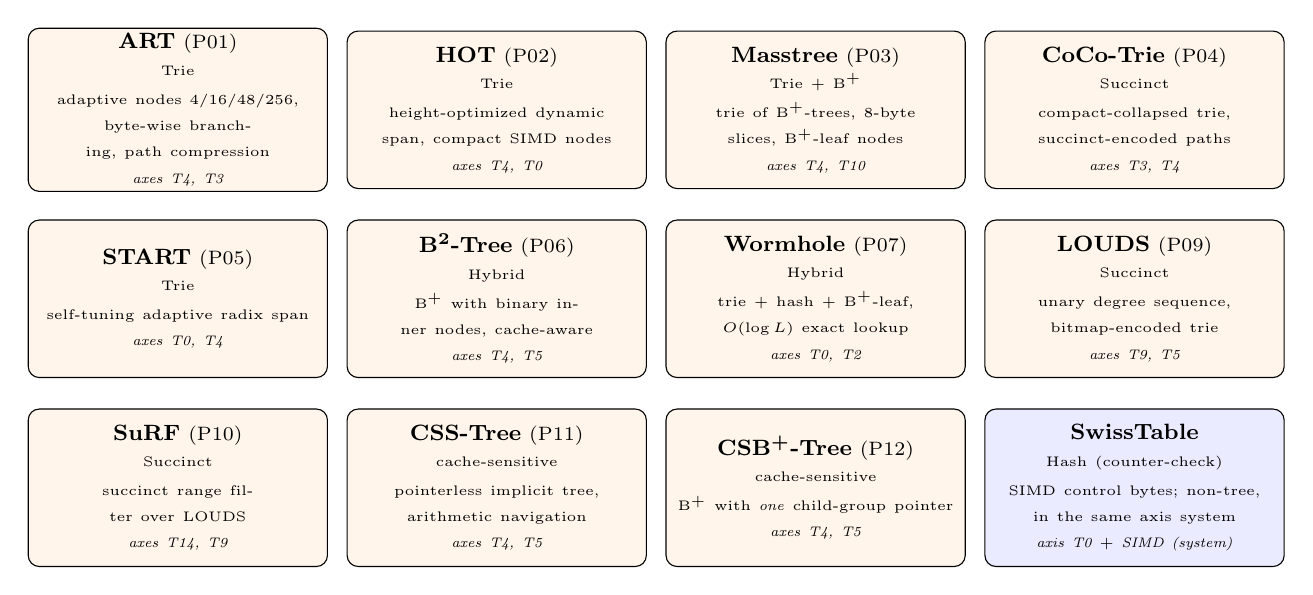
\begin{tikzpicture}[font=\footnotesize,
  so/.style={draw,rounded corners,fill=orange!8,minimum width=3.8cm,minimum height=2.0cm,text width=3.55cm,align=center,inner sep=2pt}]
  \node[so] (a1) at (0,0){\textbf{ART} {\scriptsize(P01)}\\{\tiny Trie}\\[1pt]{\tiny adaptive nodes 4/16/48/256, byte-wise branching, path compression}\\{\tiny\itshape axes T4, T3}};
  \node[so] (a2) at (4.05,0){\textbf{HOT} {\scriptsize(P02)}\\{\tiny Trie}\\[1pt]{\tiny height-optimized dynamic span, compact SIMD nodes}\\{\tiny\itshape axes T4, T0}};
  \node[so] (a3) at (8.1,0){\textbf{Masstree} {\scriptsize(P03)}\\{\tiny Trie $+$ B\textsuperscript{+}}\\[1pt]{\tiny trie of B\textsuperscript{+}-trees, 8-byte slices, B\textsuperscript{+}-leaf nodes}\\{\tiny\itshape axes T4, T10}};
  \node[so] (a4) at (12.15,0){\textbf{CoCo-Trie} {\scriptsize(P04)}\\{\tiny Succinct}\\[1pt]{\tiny compact-collapsed trie, succinct-encoded paths}\\{\tiny\itshape axes T3, T4}};
  \node[so] (b1) at (0,-2.4){\textbf{START} {\scriptsize(P05)}\\{\tiny Trie}\\[1pt]{\tiny self-tuning adaptive radix span}\\{\tiny\itshape axes T0, T4}};
  \node[so] (b2) at (4.05,-2.4){\textbf{B\textsuperscript{2}-Tree} {\scriptsize(P06)}\\{\tiny Hybrid}\\[1pt]{\tiny B\textsuperscript{+} with binary inner nodes, cache-aware}\\{\tiny\itshape axes T4, T5}};
  \node[so] (b3) at (8.1,-2.4){\textbf{Wormhole} {\scriptsize(P07)}\\{\tiny Hybrid}\\[1pt]{\tiny trie $+$ hash $+$ B\textsuperscript{+}-leaf, $O(\log L)$ exact lookup}\\{\tiny\itshape axes T0, T2}};
  \node[so] (b4) at (12.15,-2.4){\textbf{LOUDS} {\scriptsize(P09)}\\{\tiny Succinct}\\[1pt]{\tiny unary degree sequence, bitmap-encoded trie}\\{\tiny\itshape axes T9, T5}};
  \node[so] (c1) at (0,-4.8){\textbf{SuRF} {\scriptsize(P10)}\\{\tiny Succinct}\\[1pt]{\tiny succinct range filter over LOUDS}\\{\tiny\itshape axes T14, T9}};
  \node[so] (c2) at (4.05,-4.8){\textbf{CSS-Tree} {\scriptsize(P11)}\\{\tiny cache-sensitive}\\[1pt]{\tiny pointerless implicit tree, arithmetic navigation}\\{\tiny\itshape axes T4, T5}};
  \node[so] (c3) at (8.1,-4.8){\textbf{CSB\textsuperscript{+}-Tree} {\scriptsize(P12)}\\{\tiny cache-sensitive}\\[1pt]{\tiny B\textsuperscript{+} with \emph{one} child-group pointer}\\{\tiny\itshape axes T4, T5}};
  \node[draw,rounded corners,fill=blue!8,minimum width=3.8cm,minimum height=2.0cm,text width=3.55cm,align=center,inner sep=2pt] (c4) at (12.15,-4.8){\textbf{SwissTable}\\{\tiny Hash (counter-check)}\\[1pt]{\tiny SIMD control bytes; non-tree, in the same axis system}\\{\tiny\itshape axis T0 $+$ SIMD (system)}};
\end{tikzpicture}
\caption{Gallery of the most important reconstructed search structures: per method (with paper ID) its origin class, the characteristic structural idea, and the axes at which it makes its main contribution. Trie, hybrid, succinct, and cache-sensitive methods stand next to a non-tree hash counter-check (SwissTable) --- all as points in the same axis design space. The complete axis dissection is given in Table~\ref{tab:axes-overview}.}\label{fig:sota-gallery}
\end{figure}

For each SOTA algorithm (\emph{state of the art} --- the state of the art from
Section~\ref{sec:overview}) and each allocator a profile XML records the axis assignment: the
organ assignment (\texttt{node}, \texttt{traversal}, \texttt{value\_handle}, \texttt{concurrency},
\texttt{allocator}, \texttt{prefetch}, \texttt{layout}, \texttt{reclamation}), the probe build axis
\texttt{page}, and --- separately from it, because not an organ assignment --- the target ISA (\texttt{isa},
system sphere) and the telemetry (\texttt{telemetry}, measurement tooling); in addition a key-value signature
and an optional \texttt{<expected\_workload>} tag that overrides the measurement heuristic
(Table~\ref{tab:sota-profiles}).

For each of the 33~corpus works and each of the 23~allocators there exists a profile XML
with \texttt{<expected\_workload>} tag. The profiles are of two types --- the type is marked in the
profile XML and anchored compile-statically in the probe registry of the cache engine: 30
\emph{full profiles} describe standalone search designs completely; three \emph{abstract profiles}
enter only dissected --- the optimistic lock coupling of ART~\cite{leis2016olc} as a
concurrency organ, the succinct LOUDS representation~\cite{jacobson1989louds} as a
memory-layout organ (e.g.\ in SuRF~\cite{zhang2018surf}), and the profiling tool
VAMPIR~\cite{berthold2023vampir} as a measurement technology. An abstract profile supplies some organs itself
and leaves the rest to the default toolkit; it is the same type that the probe PRT-ART
corresponds to (Section~\ref{sec:prtart-demo}), and full profiles of foreign probes can be integrated
along the same path. The design envisions per axis a separate permutation over
\emph{profile ranges} --- a value range per axis instead of a single value; the persisted
profiles contain a single value per axis, the range permutation is not implemented.

\begin{table}[!htbp]
  \caption{SOTA profiles (33: 30 full profiles, 3 abstract) with workload affinity}\label{tab:sota-profiles}
  \centering\small
  \begin{tabular}{llll}
    \toprule
    \textbf{Profile} & \textbf{Paper ref.} & \textbf{Type} & \textbf{expected\_workload} \\
    \midrule
    art & P01 (Leis 2013) & full & YCSB\_C \\
    hot & P02 (Binna 2018) & full & YCSB\_C \\
    masstree & P03 (Mao 2012) & full & YCSB\_A \\
    coco\_trie & P04 (Boffa 2024) & full & YCSB\_C \\
    start & P05 (Fent 2020) & full & YCSB\_C \\
    b2tree & P06 (Schmeisser 2022) & full & YCSB\_E \\
    wormhole & P07 (Wu 2019) & full & YCSB\_A \\
    olc & P08 (Leis 2016) & abstract & YCSB\_B \\
    louds & P09 (Jacobson 1989) & abstract & YCSB\_A \\
    surf & P10 (Zhang 2018) & full & YCSB\_A \\
    css\_tree & P11 (Rao/Ross 1999) & full & YCSB\_C \\
    csb\_tree & P12 (Rao/Ross 2000) & full & YCSB\_E \\
    hankins & P13 (Hankins 2003) & full & YCSB\_C \\
    samuel & P14 (Samuel 2005) & full & YCSB\_C \\
    graefe & P15 (Graefe 2001) & full & YCSB\_C \\
    bender\_treelayout & P16 (Bender 2002) & full & YCSB\_C \\
    bender\_cacheoblivious & P17 (Bender 2005) & full & YCSB\_C \\
    saikkonen\_multilevel & P18 (Saikkonen 2008) & full & YCSB\_E \\
    saikkonen\_layoutinvariant & P19 (Saikkonen 2016) & full & YCSB\_E \\
    btreesareback & P20 (Mueller 2025) & full & YCSB\_E \\
    chen\_prefetch & P21 (Chen 2001) & full & YCSB\_A \\
    chen\_fractal & P22 (Chen 2002) & full & YCSB\_A \\
    khan\_adaptive & P23 (Khan 2010) & full & YCSB\_A \\
    naderan\_tahan & P24 (Naderan-Tahan 2016) & full & YCSB\_A \\
    mahling & P25 (Mahling 2025) & full & YCSB\_E \\
    zhang\_fgcs & P26 (Zhang 2024) & full & YCSB\_A \\
    zhang\_asplos & P27 (Zhang 2025) & full & YCSB\_A \\
    kuehn & P28 (Kuehn 2023) & full & YCSB\_C \\
    rcu & P29 (McKenney 2001) & full & YCSB\_B \\
    hazard\_pointers & P30 (Michael 2004) & full & YCSB\_B \\
    ungethuem & P31 (Ungethuem 2017) & full & YCSB\_C \\
    to\_stride & P32 (Schmidt 2025) & full & YCSB\_C \\
    vampir & P33 (Berthold 2023) & abstract & YCSB\_B \\
    \bottomrule
  \end{tabular}

  \smallskip
  {\footnotesize \texttt{expected\_workload} = YCSB workload class (A/B/C/E/F); type: full = full profile of a
  standalone search design, abstract = abstract profile that enters only dissected.\par}
\end{table}

Across all 33 profiles these affinities distribute into 13$\times$~YCSB\_C (read-heavy),
10$\times$~YCSB\_A (zipf-distributed read and update), 6$\times$~YCSB\_E (range scans), and
4$\times$~YCSB\_B (95/5 read/update); PRT-ART itself is tagged in its probe profile with YCSB\_F
(read-modify-write, for the DensityTracker updates).

The core finding of this load-profile analysis is a systematic \emph{bias}: each publication chooses
the load profile under which its own design performs best. Static, read-only-oriented
tries and filters (HOT~\cite{binna2018hot}, CoCo~\cite{boffa2024coco},
B\textsuperscript{2}-tree~\cite{schmeisser2022b2tree}, SuRF~\cite{zhang2018surf}, CSS~\cite{rao1999css})
frame \enquote{build-once, 100\,\% positive lookups} and avoid updates; compressed tries and
filters (CoCo, B\textsuperscript{2}-tree, SuRF) make the negative-query share the primary axis, because they
abort early on misses; zipfian-centred works (B-Trees Are Back~\cite{mueller2025btreesback},
Mahling~\cite{mahling2025hotpath}, Kuehn~\cite{kuehn2023bplustree}) favour cache-aware
reordering layouts; write- and concurrency-heavy works (ART~\cite{leis2013art},
Masstree~\cite{mao2012masstree}, Wormhole~\cite{wu2019wormhole}, OLC-ART~\cite{leis2016olc},
RCU~\cite{mckenney2001rcu}) conversely compete only where static structures fail; and prefetch-
and hardware-near works (CSB\textsuperscript{+}~\cite{rao2000csb}, Chen~\cite{chen2001prefetch},
Schmidt~\cite{schmidt2025hbm}) measure, via node size and prefetch, cache and TLB rather than the
algorithm logic. Fourteen of the publications contribute no distinct load profile to the catalogue ---
partly survey, theory, and hardware works without an index load profile of their own, partly works whose
custom microbenchmarks are subsumed by profiles already catalogued. Only when \emph{all} load profiles
run against \emph{all} living-being binaries (and the container hulls, Section~\ref{sec:anatomy-levels})
--- the workload as a dynamic axis
(Chapter~\ref{ch:eval}) --- can an advantage that exists only under the self-chosen load profile
be made visible and bias-reduced comparability be gained.

Finally, the quality criteria of scientific measurement (cf.\ the definitional classes in Section~\ref{sec:measurement-system}), too, appear
as concrete technologies.\ \emph{Hardware performance counters} (PMC, via \texttt{perf})~\cite{demelo2010perf}
are nearly universal and deliver cache-miss rates, dTLB misses, branch misses, and IPC/CPI --- the
majority of the works P01--P28 report such counters ---; \emph{profilers}
such as OTF2/VAMPIR~\cite{berthold2023vampir} and VTune~\cite{reinders2005vtune} collect trace-based
runtime profiles, \emph{simulators} such as gem5~\cite{binkert2011gem5} provide hardware-accurate estimates where
real counters are absent (so P25 Mahling~\cite{mahling2025hotpath}, P27
Zhang~\cite{zhang2025hierarchical}), and the \emph{HdrHistogram}~\cite{tene_hdrhistogram} collects the latency
percentiles (p50/p95/p99). On the collection the evaluation builds: instead of arithmetic means, median and
percentiles are reported, differences tested for significance with the distribution-free \emph{Mann-Whitney U test}~\cite{mann1947utest}
(with Holm correction of the family-wise error rate~\cite{holm1979sequential}) and quantified via the effect measure
\emph{Cliff's~$\delta$}~\cite{cliff1993dominance}, following the recommendations for scientific
benchmarking~\cite{hoefler2015benchmarking}. A methodological line of its own is the hardware-near
measurement methodology of TU Dresden (Habich group): Ungethüm et al.~\cite{ungethuem2017survey} systematize the
hardware optimizations for database machines, Schmidt et al.~\cite{schmidt2025hbm} measure stride versus
sequential accesses on HBM with dTLB and L2/L3 counters, and VAMPIR~\cite{berthold2023vampir} profiles non-functional properties
of heterogeneous memory. From all these technologies follows the set of measurement categories ---
cache-line utilization, cache misses (L1/L2/L3), dTLB misses, memory footprint, branch misses,
IPC/CPI, latency (mean and percentiles p50--p999), throughput, energy, and fill-buffer occupancy ---,
whose time- and observer-based subset the present apparatus already resolves (wall clock,
HdrHistogram in the downstream evaluation, per-axis observers, the statistics triad of
median/percentiles, significance test, and effect measure, the two-phase operation loop, and the
conformance gate against \texttt{std::map}),
while the counter-based PMC categories are mandatorily built into the measurement path and their assignment per
microarchitecture is bound to an event catalogue (Section~\ref{sec:axis-triad}); the
complete measurement architecture is developed by the measurement system (Section~\ref{sec:measurement-system})
and Chapter~\ref{ch:eval}.

\section{Solution Concept: the Anatomy Model}\label{sec:anatomy-model}
From the dialectical adoption of the state of the art emerges the solution concept of this thesis;
this section develops it as the \emph{anatomy model} and in doing so defines the terminology and
conceptual special constructs on which the following sections build.

\subsection{Axis Composition and the Living-Being Metaphor}\label{sec:anatomy-metaphor}
The central idea is to treat an algorithm not as a monolith but as a \emph{composition of orthogonal
axes} --- each axis a partial decision of a cache-aware or system-aware index (how pages are
arranged, how nodes branch, how memory is allocated). A concrete algorithm is then
a point in the Cartesian product of all axes, a state-of-the-art design an explicit
configuration. The decisive property is \emph{modular exchangeability}: a new axis variant can be
studied in isolation --- its effect measured per axis \emph{and} for the whole algorithm --- without
reimplementing the others; this is precisely what solves the separability problem, since the contribution of each constituent
becomes measurable in isolation while the other axes are held fixed. That this exchangeability is modular shows in the
code: the reference compositions of ART and PRT-ART differ in exactly one axis, the
path compression (Section~\ref{sec:prtart-demo}). This decomposition rests on the observation of shared concerns of different search algorithms and publications, as well as on the comparability of the goals of different search algorithms, and can therefore be carried by a metaphor. First,
search algorithms share, in the large, the same \emph{tree anatomy} in different expressions ---
from balanced search trees through tries and radix trees to custom constructs; even a
sorted key--value list is, strictly speaking, a single leaf of a tree whose values point onward via
references to data leaves. The main differences between the algorithm expressions thereby come down to the fan-out of the nodes, the tree depth, the tree filters and rule sets, and the implementation details of the serialization of memory pages, search pages, and tree nodes. The tree structure is thus universal across all search-algorithm architectures and forms the canvas on which the axes are placed.

Non-tree-like search methods --- such as the hash counter-check of Section~\ref{sec:sota-instances} ---
remain the same family with a restricted profile, for a separate family would arise only if the
base axis set differed fundamentally: a hash table, too, is a tree that searches from the root
of its interface over a fan-out of hashes --- only the core algorithm of the node is a
different one. Therefore every method that translates a key into a value, no matter how, belongs to the
family Map and its genus \texttt{SearchAlgorithm} (Section~\ref{sec:anatomy-levels}). Second,
a vivid metaphor treats a concrete algorithm as a \emph{living being} whose
\emph{organs} are the axes. The metaphor is canonically cast: the \emph{blood} is the liquid
organ that connects all organ axes and is condensed in the planner into a compile-time configuration;
the system axes are the \emph{habitat} (the planet) of the animal with the possibilities and
resources found there; the measurement axes are the equipment of the \emph{laboratory} in which the
animal is examined (Figure~\ref{fig:anatomy-bridge}). An animal can live very well without measurement,
but only the healthiest animal shall be put into productive use --- and every animal shall be
adapted as well as possible to its habitat: if it lacks a property, it cannot use this part of
its habitat (the hardware) to its advantage; or the measurement finds out that its
specialization should not be geared to this habitat at all, because it negatively affects the quality of the animal
there --- a monkey shall climb and a fish shall swim, not the other way round, because
different objectives have led to different designs. This metaphor is owed to the
author's background in biomedical engineering and is meant to ease the analysis through
vividness; from here on the thesis works consistently with this model.

\begin{figure}[htbp]\centering
\begin{tikzpicture}[font=\footnotesize, align=center, >=Stealth,
  organism/.style={draw, rounded corners, minimum width=2.8cm, minimum height=3.4cm, fill=red!4},
  org/.style={draw, circle, fill=red!15, minimum size=0.78cm, inner sep=0pt, font=\scriptsize},
  axis/.style={draw, rounded corners, fill=green!10, minimum width=2.2cm, minimum height=0.55cm, font=\scriptsize},
  habitat/.style={draw, rounded corners, fill=yellow!16, minimum height=0.7cm, text width=7.8cm, font=\scriptsize}]
  \node[organism] (body) at (0,-0.1){};
  \node[font=\scriptsize] at (0,1.95){\textbf{living being} (anatomy)};
  \node[org] (o1) at (0,0.9){heart};
  \node[org] (o2) at (-0.65,-0.1){lung};
  \node[org] (o3) at (0.65,-0.1){liver};
  \node[org] (o4) at (0,-1.1){kidney};
  \draw[->,very thick] (1.7,-0.1) -- (3.0,-0.1) node[midway,above,font=\scriptsize]{organ $\equiv$ axis};
  \node[font=\scriptsize] at (5.4,1.95){\textbf{search algorithm} (axes)};
  \node[axis] (a1) at (5.4,0.9){traversal};
  \node[axis] (a2) at (5.4,0.2){layout};
  \node[axis] (a3) at (5.4,-0.5){allocator};
  \node[axis] (a4) at (5.4,-1.2){prefetch};
  \draw[red!60!black,thick] (4.15,1.15) -- (4.15,-1.45);
  \foreach \y in {0.9,0.2,-0.5,-1.2}{\draw[red!60!black,thick] (4.15,\y) -- (4.3,\y);}
  \node[font=\tiny,text=red!60!black,rotate=90] at (3.95,-0.15){blood $=$ connection of the organ axes};
  \node[habitat,minimum width=8.2cm] (hab) at (2.7,-2.45){\textbf{habitat} (system axes): the planet with its resources --- always present, belonging to no family};
  \node[draw, fill=blue!8, font=\scriptsize, align=center] (mess) at (8.3,-0.15){measurement system\\(\enquote{laboratory})};
  \draw[->,blue] (mess) -- (a1); \draw[->,blue] (mess) -- (a2);
  \draw[->,blue] (mess) -- (a3); \draw[->,blue] (mess) -- (a4);
\end{tikzpicture}
\caption{The anatomy bridge: just as a living being consists of interacting organs, a search algorithm is a composition of axis-organs; the blood connects the organ axes, the habitat (the system axes) carries the animal, and the measurement system takes the role of the laboratory that measures each organ in isolation.}\label{fig:anatomy-bridge}
\end{figure}

The permutation of the axes is, in this reading, an organ exchange: exchanging organs between
living beings produces new composite algorithms with hitherto unknown cache-line behaviour. The organs themselves
are won from the state of the art --- the design building blocks of the known methods
(Section~\ref{sec:overview}) are decomposed into orthogonal axes and collected in a shared
axis matrix, so that each axis harvests the contributions of the entire corpus
(Figure~\ref{fig:synth}).
\begin{figure}[htbp]\centering
\begin{tikzpicture}[font=\footnotesize,>=Stealth,align=center,
  paper/.style={draw,rounded corners,fill=orange!12,minimum width=1.8cm,minimum height=0.52cm},
  ax/.style={draw,fill=green!12,minimum width=2.2cm,minimum height=0.5cm,font=\scriptsize}]
  \node[font=\scriptsize,text=gray] at (0,2.95){state of the art};
  \node[paper] (p1) at (0,2.2){ART};
  \node[paper] (p2) at (0,1.5){HOT};
  \node[paper] (p3) at (0,0.8){SuRF};
  \node[paper] (p4) at (0,0.1){Masstree};
  \node[paper] (p5) at (0,-0.6){Bw-tree};
  \node[font=\scriptsize,text=gray] at (5.6,2.95){the axis matrix};
  \node[ax] (x1) at (5.6,2.2){node type};
  \node[ax] (x2) at (5.6,1.5){layout};
  \node[ax] (x3) at (5.6,0.8){allocator};
  \node[ax] (x4) at (5.6,0.1){prefetch};
  \node[ax] (x5) at (5.6,-0.6){concurrency};
  \foreach \p in {p1,p2,p3,p4,p5}{\foreach \x in {x1,x2,x3,x4,x5}{\draw[gray!22,->] (\p.east)--(\x.west);}}
  \node[align=center,font=\scriptsize] at (2.8,-1.7){every algorithm decomposes into axis assignments ---\\the matrix harvests the building blocks of the whole corpus};
\end{tikzpicture}
\caption{Synthesis state of the art $\to$ axes: the design building blocks of the known methods are decomposed into orthogonal axes; each axis collects the contributions of the entire corpus --- the inverse of Figure~\ref{fig:design-space} (there an algorithm is a point, here an axis is a collecting basin).}\label{fig:synth}
\end{figure}

The \emph{anatomy} thus won is more than the enumeration of the organs: it is their \emph{wiring}.
Each organ exports a generalized interface through which the others use its services without
knowing its concrete assignment --- thus the allocation organ provides a shared
allocation interface that node layout, value placement, and serialization use for their
memory needs (Figure~\ref{fig:axis-organ}); the hub of this wiring is in the code
the storage organ \texttt{LayoutAwareChunkedStore}, which composes node type, layout, and allocator
(\enquote{storage-organ interface} is the concept name, not a code type). The usage rules are broadly
drawn: an axis may use foreign axis interfaces, call itself recursively, and use other
families --- the search family accesses axes in its interface functions and uses
container genera of its own, and parts of the axis pool are reused for the containers
(Section~\ref{sec:measurement-system}). In software-engineering terms this is the \emph{feature interaction}
of feature-oriented software product lines~\cite{apel2013feature,batory1992hierarchical}.

An axis corresponds to a feature, a living being to a feature composition. The \emph{family} is the
feature \emph{core} composition: the shared interface core that all genera of a family share and
that is used identically in the metaprogramming across all variations --- just as different
map categories (hash map, flat map) share a common core of interface functions; for the
container family this core consists of identity, axis observation, and size. The \emph{genus}
(alias: tier subclass, Section~\ref{sec:anatomy-levels}) is the feature \emph{special} composition:
the real tier interface beyond the core --- \texttt{SearchAlgorithm}, \texttt{Set},
\texttt{Sequence}, \texttt{Adapter}, \texttt{View}, and \texttt{FunctionInterfaceReroute} --- and thus
a static feature-set definition. The anatomy is the wiring between the features. Which
axis uses which is shown by the inter-organ usage graph (Figure~\ref{fig:usage}).
\begin{figure}[htbp]\centering
\begin{tikzpicture}[font=\footnotesize,>=Stealth,align=center,
  organ/.style={draw,circle,minimum size=1.05cm,fill=green!7,inner sep=1pt}]
  \node[organ,fill=blue!12,minimum size=1.3cm] (store) at (0,0){storage\\organ};
  \node[organ] (alloc) at (-3.0,1.5){allocator};
  \node[organ] (node) at (-3.0,0){node type};
  \node[organ] (layout) at (-3.0,-1.5){layout};
  \node[organ] (search) at (3.0,0){search};
  \node[organ,fill=gray!8] (obs) at (2.8,-2.3){telemetry};
  \draw[->,thick,blue] (alloc)--(store);
  \draw[->,thick,blue] (node)--(store);
  \draw[->,thick,blue] (layout)--(store);
  \draw[->,thick,blue] (store)--(search) node[midway,above,font=\scriptsize,text=blue]{must};
  \draw[->,dashed,gray] (store)--(obs) node[midway,right,font=\scriptsize]{can};
  \node[font=\scriptsize,blue] at (0,-1.6){storage-organ interface\\{\tiny (\texttt{LayoutAwareChunkedStore})}};
\end{tikzpicture}
\caption{Axis $=$ organ, anatomy $=$ wiring: the storage organ (composition of node type, layout, and allocator) exports a generalized storage-organ interface (in the code \texttt{LayoutAwareChunkedStore}) over which the search runs (solid, \emph{mandatory}); further organs such as the telemetry \emph{can} use it via optional observer hooks (dashed, \emph{optional}), but need not.}\label{fig:axis-organ}
\end{figure}

Composing these pairwise \emph{organ couplings} --- an organ coupling is the mutual
dependency of two axes in which the one uses the interface of the other (mandatorily or
optionally) or restricts its admissible assignments; sub-question RQ1.b (Section~\ref{sec:rqs})
addresses it for node type, SIMD, and path compression --- across all organs together yields a
directed inter-organ usage graph.
\begin{figure}[htbp]\centering
% No \resizebox: the drawing is only ~10.3cm wide; blowing it up to \linewidth (x1.55) would inflate
% the \scriptsize font beyond the body text. Rule: resizebox only to SHRINK (cf. fig:m-model).
\begin{tikzpicture}[font=\footnotesize,>=Stealth,align=center,
  org/.style={draw,rounded corners,fill=green!8,minimum width=2.1cm,minimum height=0.66cm,font=\scriptsize},
  hub/.style={draw,rounded corners,fill=blue!12,minimum width=3.2cm,minimum height=1.15cm,text width=3.0cm,align=center,font=\scriptsize,very thick}]
  \node[hub] (store) at (0,0){\textbf{storage organ}\\\texttt{Layout\-Aware\-Chunked\-Store}\\{\scriptsize T4\,$\oplus$\,T5\,$\oplus$\,T6}};
  \node[org] (alloc) at (-4.1,1.4){allocator (T6)};
  \node[org] (node) at (-4.1,0){node type (T4)};
  \node[org] (layout) at (-4.1,-1.4){layout (T5)};
  \node[org] (search) at (4.1,0){search (T0)};
  \node[org] (prefetch) at (4.1,1.4){prefetch (T7)};
  \node[org,fill=gray!8] (obs) at (4.1,-1.4){telemetry (meas.)};
  \node[org,fill=gray!6] (conc) at (0,-2.6){concurrency (T8)};
  \draw[->,very thick,blue] (alloc)--(store);
  \draw[->,very thick,blue] (node)--(store);
  \draw[->,very thick,blue] (layout)--(store);
  \draw[->,very thick,blue] (store)--(search) node[midway,above,font=\scriptsize]{must};
  \draw[->,dashed,gray] (store)--(prefetch) node[midway,above,font=\scriptsize]{can};
  \draw[->,dashed,gray] (store)--(obs);
  \draw[->,dotted,gray] (conc)--(store);
\end{tikzpicture}
\caption{Inter-organ usage graph (\enquote{which axis uses which}): there is exactly \emph{one}
canonical hub --- the storage organ \texttt{LayoutAwareChunkedStore}, which composes node type~(T4), layout~(T5),
and allocator~(T6)\@. \emph{Mandatorily} (solid) the store consumes these three axes,
and the search~(T0) runs over it. All remaining couplings are \emph{optional} (dashed): prefetch~(T7)
and the telemetry (measurement instrumentation, Section~\ref{sec:axis-triad}) read the store only via \texttt{requires}-gated observer hooks --- an axis
\emph{can} use foreign interfaces, but \emph{need} not. The coupling of concurrency~(T8) to the
store is not connected (dotted). The graph is an example wiring of the storage organ,
not a structure evaluated in the code.}\label{fig:usage}
\end{figure}
\subsection{The Three-Level Model and the Four Families}\label{sec:anatomy-levels}
These organs are embedded in \emph{one} architecture --- a single, self-contained hierarchy
without parallel trees. At its root stands the \texttt{ExecutionEngine} as the common, measurable
abstraction over everything measurable --- it persists because \texttt{IExecutionEngine} forms the
common measurable root and \texttt{IAnatomyBase} the anatomy-bearing view immediately beneath it;
beneath that, three levels can be distinguished: the \emph{family} as the outward-visible
algorithm interface (the \emph{probe dock}), beneath it the \emph{genus} (alias: \emph{tier subclass})
with a fixed axis set, beneath that the \emph{organs} themselves (Figure~\ref{fig:three-levels})\@. The
separation of levels can be read off at the ABI boundary: every tier binary exports two letter-identical
C symbols that answer family and genus without an instance, whereby the family is not maintained as a second datum
but derived from the genus --- the loader thus determines the family via a
family-independent symbol, without knowing it in advance\@. \enquote{Living being} and \texttt{SearchAlgorithm} denote the same
entity --- metaphor and technical term ---; the anatomy is not a second model but the
\emph{body} of this living being: the fixed composition of its eighteen axis-organs.
\begin{figure}[htbp]\centering
\begin{tikzpicture}[font=\footnotesize,>=Stealth,align=center,
  box/.style={draw,rounded corners,inner sep=3pt,minimum height=0.7cm},
  lvl/.style={font=\scriptsize,text=gray,anchor=east,align=right}]
  \node[box] (root) at (1.1,0){\texttt{IExecutionEngine} (measurable root) $\to$ \texttt{IAnatomyBase} (anatomy-bearing)};
  \node[lvl] at (-5.1,-1.6){Level 1: family\\{\tiny feature core composition}};
  \node[box] (sa) at (-3.0,-1.6){Map};
  \node[box] (co) at (0,-1.6){Container};
  \node[box] (gr) at (2.6,-1.6){Graph};
  \node[box] (ha) at (5.3,-1.6){HeuristikAdapter};
  \node[lvl] at (-5.1,-3.3){Level 2: genus\\{\tiny feature special composition}};
  \node[box] (tier) at (-3.0,-3.3){\texttt{SearchAlgorithm}\\{\scriptsize mammal, 18 organ axes}};
  \node[box] (cont2) at (0,-3.3){\texttt{Set}, \texttt{Sequence},\\\texttt{Adapter}, \texttt{View}};
  \node[box,dashed,fill=gray!8] (gr2) at (2.6,-3.3){no genus\\{\scriptsize implemented}};
  \node[box] (ha2) at (5.3,-3.3){\texttt{FunctionInterface}-\\\texttt{Reroute}};
  \node[lvl] at (-5.1,-4.75){Level 3: organs};
  \node[box,fill=green!8] (org) at (-3.0,-4.75){axes T0--T17};
  \node[box,fill=green!8] (org2) at (0,-4.75){axes of the pool};
  \draw[->] (root)--(sa);\draw[->] (root)--(co);\draw[->] (root)--(gr);\draw[->] (root)--(ha);
  \draw[->] (sa)--(tier);\draw[->] (co)--(cont2);\draw[->,dashed] (gr)--(gr2);\draw[->] (ha)--(ha2);
  \draw[->] (tier)--(org);\draw[->] (cont2)--(org2);
\end{tikzpicture}
\caption{The three-level model: family (level~1, outer interface, feature core composition) $\to$ genus (level~2, fixed axis set, feature special composition) $\to$ organs/axes (level~3). Four families: \texttt{Map} possesses as its sole genus \texttt{SearchAlgorithm}, the \enquote{mammal} with the eighteen organ axes; \texttt{Container} the genera Set/Sequence/Adapter/View, which are formed from the same axis pool; \texttt{Graph} is laid out as an interface, a genus is not implemented; \texttt{HeuristikAdapter} possesses the reroute genus \texttt{FunctionInterfaceReroute} of the hybrid tier.}\label{fig:three-levels}
\end{figure}

At the topmost level stand four families. The \texttt{Map} family --- the
key-value-oriented probe dock and the focus of this thesis --- possesses as its sole genus
\texttt{SearchAlgorithm}, the full eighteen-axis \enquote{mammal}; the \texttt{Container} family
(keyless storage) fans out into the genera Set, Sequence, Adapter, and View, which are likewise formed from
axes of the shared pool and whose slot count per genus is fixed
compile-statically; the \texttt{Graph} family is laid out as an interface, a genus is not implemented; and
the \texttt{HeuristikAdapter} family possesses the reroute genus \texttt{FunctionInterfaceReroute} --- the
family of the hybrid tier (Section~\ref{sec:heuristics-modes}), which by metaprogramming inherits the
interfaces of a family together with a genus and passes requests through to the actual tier binaries;
classification (of which kind the reroute is) and pass-through (the inherited target genus that the binary
reports outwardly) lie on separate levels (Figure~\ref{fig:genera}). Mnemonic:
\enquote{Adapter} without prefix always means the container genus; the hybrid family is always called
HeuristikAdapter. The kingdom \enquote{Animalia} ($\equiv$ \texttt{IAnatomyBase}) shown there as the root
is the anatomy-bearing view immediately beneath the measurable root \texttt{IExecutionEngine} of
Figure~\ref{fig:three-levels}; the code separation of the two interfaces is deepened in Chapter~\ref{ch:impl}.
Non-tree-like methods thus require no family of their own but occupy a restricted
axis subset of the same family.
\begin{figure}[htbp]\centering
% No \resizebox: the drawing is only ~14cm wide; blowing it up to \linewidth would inflate
% the \scriptsize font beyond the body text. Rule: resizebox only to SHRINK (cf. fig:m-model).
\begin{tikzpicture}[font=\footnotesize,>=Stealth,align=center,
  gen/.style={draw,rounded corners,fill=blue!10,minimum width=2.5cm,minimum height=0.66cm,font=\bfseries\footnotesize},
  sub/.style={draw,fill=green!8,minimum width=2.8cm,minimum height=0.62cm,font=\scriptsize},
  tbd/.style={draw,dashed,fill=gray!12,minimum width=2.5cm,minimum height=0.7cm,font=\scriptsize},
  band/.style={draw,rounded corners,fill=orange!9,minimum width=13.6cm,minimum height=1.05cm,text width=13.2cm,align=left,font=\scriptsize}]
  \node[draw,rounded corners,fill=red!6,font=\footnotesize] (root) at (1.3,1.6){kingdom \enquote{Animalia} ($\equiv$ \texttt{IAnatomyBase}, anatomy-bearing)};
  % Level 1 --- families (outer interface)
  \node[gen] (g1) at (-4.0,0){Map};
  \node[gen] (g2) at (0.6,0){Container};
  \node[gen] (g3) at (4.3,0){Graph};
  \node[gen,minimum width=2.9cm] (g4) at (7.4,0){HeuristikAdapter};
  \draw[->] (root)--(g1); \draw[->] (root)--(g2); \draw[->] (root)--(g3); \draw[->] (root)--(g4);
  % Level 2 --- genera (tier subclasses)
  \node[sub,fill=green!18] (s1) at (-4.0,-1.3){\textbf{mammal} $=$ \texttt{SearchAlgorithm}\\{\scriptsize \texttt{map} hull $\cdot$ 18 organ axes}};
  \node[sub,anchor=west] (c1) at (-1.2,-1.15){bird $=$ Set {\scriptsize(\texttt{set})}};
  \node[sub,anchor=west] (c2) at (-1.2,-1.95){reptile $=$ Sequence {\scriptsize(\texttt{vector})}};
  \node[sub,anchor=west] (c3) at (-1.2,-2.75){invertebrate $=$ Adapter {\scriptsize(\texttt{stack})}};
  \node[sub,anchor=west] (c4) at (-1.2,-3.55){plant $=$ View {\scriptsize(\texttt{span})}};
  \node[tbd,text width=2.4cm,anchor=north] (gr1) at (4.3,-0.7){interface laid out,\\{\scriptsize no genus}\\{\scriptsize implemented}};
  \node[sub,minimum width=2.9cm,text width=2.9cm,anchor=north] (h1) at (7.4,-0.7){\texttt{FunctionInterface}\\\texttt{Reroute}\\{\scriptsize hybrid tier:}\\{\scriptsize inherited target genus}};
  \draw[->] (g1)--(s1); \draw[->,dashed] (g3)--(gr1); \draw[->] (g4)--(h1);
  \draw (g2.south) -- ++(0,-0.3) -| (-1.5,-3.55);
  \draw[->] (-1.5,0 |- c1.west) -- (c1.west); \draw[->] (-1.5,0 |- c2.west) -- (c2.west);
  \draw[->] (-1.5,0 |- c3.west) -- (c3.west); \draw[->] (-1.5,0 |- c4.west) -- (c4.west);
  % Levels 3--5 --- mammal branch down to the compiled individual
  \node[band] (l3) at (1.3,-4.75){\textbf{Level 3 --- organs:} the 18 organ axes (node type, layout, allocator, prefetch, \dots) \emph{permute}; the container genera are formed from the same axis pool.};
  \node[band] (l4) at (1.3,-6.15){\textbf{Level 4 --- concrete animal:} one assignment of \emph{all} axes $=$ one individual (ART, HOT, Masstree, SuRF, START, Wormhole, \dots; 30 full profiles) --- an abstract profile (PRT-ART, OLC, LOUDS, VAMPIR) assigns only some axes itself.};
  \node[band,fill=orange!20,very thick,minimum height=1.25cm] (l5) at (1.3,-7.7){\textbf{Level 5 --- tier binary (carrier stage):} compiled per permutation to \texttt{comdare\_perm\_\-<fp>.dll}\,/\,\texttt{.so}, refined by the probe build axis page type; the platform is stamped by the three system axes, the measurement choice by the measurement line; every tier binary offers the three interface surfaces (Figure~\ref{fig:traeger-flaechen}).};
  \draw[->,thick] (s1.south) -- (s1.south |- l3.north);
  \draw[->,thick] (l3.south) -- (l4.north); \draw[->,thick] (l4.south) -- (l5.north);
\end{tikzpicture}
\caption[The four families and the tier hierarchy down to the compiled binary]{The family/tier hierarchy across five levels. \texttt{Map}, \texttt{Container}, \texttt{Graph}, and \texttt{HeuristikAdapter} are the four \emph{families} (level~1, outer interface). Each family hosts its \emph{own} genera (level~2, alias tier subclasses): \texttt{Map} exclusively the \enquote{mammal} (genus \texttt{SearchAlgorithm}, full eighteen-axis anatomy), \texttt{Container} every \emph{non}-mammal genus (bird/reptile/invertebrate/plant $=$ Set/Sequence/Adapter/View), \texttt{Graph} a laid-out interface without an implemented genus, \texttt{HeuristikAdapter} the reroute genus of the hybrid tier. The mammal branch is drawn out down to the individual: the eighteen axis organs (level~3) permute into a concrete axis composition $=$ one concrete animal (level~4, e.g.\ ART, HOT, Masstree), which is compiled per permutation into a standalone tier binary (level~5, the carrier stage of the tier binary, additionally refined by the probe build axis page type and platform-stamped by the three system axes, Section~\ref{sec:axis-triad})\@. \emph{Every tier binary is thus an animal of its own with an actual binary genus interface and three interface surfaces}; the hierarchy reaches from the family down to the single compiled permutation. Cf.\ the condensed model in Figure~\ref{fig:three-levels}.}\label{fig:genera}
\end{figure}

The anatomy is carried by four \emph{carrier stages}: the planner, the
\emph{CacheEngineBuilder} (CEB) --- the measurement tool that the planner generates per target platform and
measurement task ---, the tier binary, and the hybrid tier binary. The planner resolves the user XML against the three
offering catalogues and chooses the measurement axes at its runtime; the CEB contains this measurement choice
compiled in, knows the platform, and permutes system and organ axes into tier binaries; the
tier binary contains the organ permutation; the hybrid tier binary additionally carries its attached
tiers. Control sits in the planner, and the chain of releases is directed: the measurement axes
determine the CEB type, the CEB defines the system axes and releases the build space, and this space
permutes system and organ axes into the tier binary. No stage passes through layers --- each
contains its layer compiled in fixedly; only the configuration travels from the XML to the finished
tier binary. The interfaces of the carriers follow a three-surface model: surface~1 is the
genus interface of a tier binary (runtime, Abstract Factory), surface~2 the stamp (compile time,
ABI-stable, Section~\ref{sec:stamp-model}), surface~3 the measurement cut-through (\texttt{IMessVisitor}), which
crosses the measurement as a seam of its own, so that family and genus interfaces remain unchanged. On tier
and hybrid tier binary all three surfaces are pronounced; planner and CEB possess the stamp surface, and
the CEB additionally carries its own measurement-gate assignment, whose coverage against the tier gates (CEB off,
tier on) is proven by a test. The contracts between planner, CEB, tier, and hybrid are distributed per stage locally
over seven stamp interfaces --- an overall self-version is carried only by the planner, measurement and
system line are carried by CEB, tier, and hybrid, the organ line only by tier and hybrid (the absence at the
CEB is the static barrier \enquote{the CEB carries no organ axes}), fingerprint and
overall stamp are carried by all four, and the attached tiers are carried only by the hybrid
(Figure~\ref{fig:traeger-flaechen}).
\begin{figure}[htbp]\centering
\begin{tikzpicture}[font=\scriptsize,>=Stealth,align=center,
  tr/.style={draw,rounded corners,fill=blue!10,minimum width=2.1cm,minimum height=0.6cm,text width=1.9cm,font=\bfseries\scriptsize},
  p/.style={draw,fill=green!18,minimum width=2.1cm,minimum height=0.48cm,text width=1.95cm,font=\tiny},
  v/.style={draw,fill=gray!10,minimum width=2.1cm,minimum height=0.48cm,text width=1.95cm,text=gray,font=\tiny},
  fl/.style={draw,rounded corners,fill=orange!10,minimum width=2.1cm,minimum height=1.25cm,text width=1.95cm,font=\tiny},
  lab/.style={anchor=east,font=\scriptsize}]
  \node[tr] (t0) at (0,0){planner};
  \node[tr] (t1) at (2.5,0){CEB};
  \node[tr] (t2) at (5.0,0){tier binary};
  \node[tr] (t3) at (7.5,0){hybrid tier};
  \draw[->,thick] (t0)--(t1); \draw[->,thick] (t1)--(t2); \draw[->,thick] (t2)--(t3);
  \node[font=\tiny,anchor=south] at (3.75,0.38){configuration travels: XML $\to$ planner $\to$ CEB $\to$ tier $\to$ hybrid (no stage passes through layers)};
  \node[lab] at (-1.2,-0.75){\texttt{version\_xyz}};
  \node[p] at (0,-0.75){mandatory}; \node[v] at (2.5,-0.75){forbidden}; \node[v] at (5.0,-0.75){forbidden}; \node[v] at (7.5,-0.75){forbidden};
  \node[lab] at (-1.2,-1.32){\texttt{mess\_zeile}};
  \node[v] at (0,-1.32){forbidden}; \node[p] at (2.5,-1.32){mandatory}; \node[p] at (5.0,-1.32){mandatory}; \node[p] at (7.5,-1.32){mandatory};
  \node[lab] at (-1.2,-1.89){\texttt{system\_zeile}};
  \node[v] at (0,-1.89){forbidden}; \node[p] at (2.5,-1.89){mandatory}; \node[p] at (5.0,-1.89){mandatory}; \node[p] at (7.5,-1.89){mandatory};
  \node[lab] at (-1.2,-2.46){\texttt{organ\_zeile}};
  \node[v] at (0,-2.46){forbidden}; \node[v,draw=red!70!black,very thick] at (2.5,-2.46){forbidden (barrier)}; \node[p] at (5.0,-2.46){mandatory}; \node[p] at (7.5,-2.46){mandatory};
  \node[lab] at (-1.2,-3.03){\texttt{fingerprint\_sha}};
  \node[p] at (0,-3.03){mandatory (SHA-256)}; \node[p] at (2.5,-3.03){mandatory (SHA-512)}; \node[p] at (5.0,-3.03){mandatory (SHA-512)}; \node[p] at (7.5,-3.03){mandatory (SHA-512)};
  \node[lab] at (-1.2,-3.60){\texttt{gesamt\_stempel}};
  \node[p] at (0,-3.60){mandatory}; \node[p] at (2.5,-3.60){mandatory}; \node[p] at (5.0,-3.60){mandatory}; \node[p] at (7.5,-3.60){mandatory};
  \node[lab] at (-1.2,-4.17){\texttt{angeschlossene}};
  \node[v] at (0,-4.17){forbidden}; \node[v] at (2.5,-4.17){forbidden}; \node[v] at (5.0,-4.17){forbidden}; \node[p] at (7.5,-4.17){mandatory (RT hook)};
  \node[lab,font=\bfseries\scriptsize] at (-1.2,-5.25){surfaces};
  \node[fl] at (0,-5.25){2 stamp\\{(version, ISA, OS $+$ SHA-256)}};
  \node[fl] at (2.5,-5.25){2 stamp (measurement choice)\\3 own measurement gates\\{(CEB off / tier on)}};
  \node[fl] at (5.0,-5.25){1 genus interface\\2 stamp\\3 measurement cut-through \texttt{IMessVisitor}};
  \node[fl] at (7.5,-5.25){1 inherited target genus\\2 stamp $+$ attached\\3 measurement cut-through};
  \node[font=\tiny,anchor=north] at (3.15,-6.25){realm lines in the metaphor: measurement line $=$ laboratory, system line $=$ habitat, organ line $=$ the organs connected by the blood};
\end{tikzpicture}
\caption{Carrier stages and interface surfaces: the three-valued admission matrix of the seven stamp interfaces over the four carrier stages planner, CacheEngineBuilder (CEB), tier binary, and hybrid tier binary (28 cells; green $=$ mandatory, grey $=$ forbidden; the cell organ line/CEB is the static barrier \enquote{the CEB carries no organ axes}) and beneath it the interface surfaces per stage --- surface~1 genus interface (runtime), surface~2 stamp (compile time, ABI-stable), surface~3 measurement cut-through. The configuration travels from the XML via planner and CEB to the tier binary; no stage passes through layers, each contains its layer compiled in.}\label{fig:traeger-flaechen}
\end{figure}

Across the carrier stages runs a \emph{run chain} of four work modes, which is registered in the
measurement realm as a sub-axis and is traversed cumulatively in fixed order:
\emph{build} builds the binaries and does not measure; \emph{measure} is the deterministic
single-thread measurement run whose result fills the measurement store; \emph{compare} reads the measurement store
with options of its own and computes which tier binary or hybrid recombination must, according to the measurement, be the
best; \emph{release} generates from that the fully optimized binary without measurement instrumentation
and re-measures its wall clock. On the hybrid level the same chain repeats synchronously
(Figure~\ref{fig:modi-kette}). There is no debug state: \texttt{--debug} is a switch of
the planner shell for the wiring check --- a flag, not a work mode. Implementation status: the
four modes are selectable and validatable and take effect on the build of the binaries; the mode-specific procedure
of compare (replay comparison instead of measuring) and release (generation of the optimal binary from the
measured values) is envisioned but not implemented --- compare and release are
selectable, validatable labels with release-equivalent build semantics.
\begin{figure}[htbp]\centering
\begin{tikzpicture}[font=\footnotesize,>=Stealth,thick,align=center,
  mode/.style={draw,rounded corners,minimum width=2.7cm,minimum height=1.15cm,text width=2.55cm,font=\scriptsize},
  built/.style={mode,fill=green!12},
  plan/.style={mode,fill=orange!12,dashed},
  lab/.style={font=\scriptsize,text=gray,anchor=east,align=right}]
  \node[lab] at (-1.55,0){tier level\\{\tiny CEB $\to$ tier binary}};
  \node[built] (b) at (0,0){\textbf{build}\\builds, does not measure};
  \node[built] (m) at (3.1,0){\textbf{measure}\\1 thread, deterministic, fills the store};
  \node[plan] (c) at (6.2,0){\textbf{compare}\\reads the store, computes the best binary};
  \node[plan] (r) at (9.3,0){\textbf{release}\\optimal binary without measurement sensors, wall clock re-measured};
  \draw[->] (b)--(m); \draw[->] (m)--(c); \draw[->] (c)--(r);
  \node[lab] at (-1.55,-2.0){hybrid level\\{\tiny repeated synchronously}};
  \node[built] (hb) at (0,-2.0){\textbf{build}};
  \node[built] (hm) at (3.1,-2.0){\textbf{measure}};
  \node[plan] (hc) at (6.2,-2.0){\textbf{compare}\\best recombination};
  \node[plan] (hr) at (9.3,-2.0){\textbf{release}\\with and without sidecar};
  \draw[->] (hb)--(hm); \draw[->] (hm)--(hc); \draw[->] (hc)--(hr);
  \draw[->,gray] (r.south) -- ++(0,-0.3) -| (hb.north);
  \node[font=\tiny,align=left,anchor=north west] at (-3.0,-2.95){green: mode selectable, validatable, and effective in the build.\\dashed/orange: mode selectable; the mode-specific procedure (replay comparison,\\generation of the optimal binary) is envisioned but not implemented.\\\texttt{--debug} is a flag of the planner shell, not a mode.};
\end{tikzpicture}
\caption{The run chain of the four work modes build $\to$ measure $\to$ compare $\to$ release as a registered sub-axis of the measurement realm, cumulative in this order and repeated synchronously on the hybrid level; compare reads the measurement store and computes the best binary or recombination, release generates the fully optimized binary without measurement sensors and re-measures its wall clock. A debug state does not exist. The assignment to the operating target pictures measurement, evaluation, working, and hybrid mode is given by Section~\ref{sec:heuristics-modes}.}\label{fig:modi-kette}
\end{figure}

\subsection{Design Patterns and Compile-Time Patterns}\label{sec:anatomy-patterns}
The actual contribution thus lies less in a single structure than in a \emph{tool}:
instead of solving the comparison problem directly, this thesis first builds this tool --- the
permutation and measurement apparatus --- with which arbitrary axis combinations can be generated and fairly
measured. Scientifically this apparatus situates itself in the software engineering of
\emph{composition}: invasive software composition from gray-box components~\cite{assmann2003invasive},
generative programming~\cite{czarnecki2000generative}, and feature-oriented
software product lines~\cite{apel2013feature,batory1992hierarchical}. The axis concept itself stems from
prior work by the author under the Comdare brand, originally for the deduplication optimization of the
UltiHash database; ComdareDB is its successor product as a concept without code, not a further entity.
The contribution of this thesis is the transfer of the principle to cache-aware search structures as
compiled, machine-optimized binaries --- its design-pattern-driven, measurement-oriented
realization. In software-engineering terms the
apparatus is a composition of named design patterns and two new compile-time patterns
(Figure~\ref{fig:patterns}).
\begin{figure}[htbp]\centering
\begin{tikzpicture}[font=\footnotesize,>=Stealth,align=center]
  \node[draw,rounded corners,fill=green!5,minimum width=12.8cm,minimum height=2.4cm] (classic) at (0,0){};
  \node[font=\bfseries\footnotesize] at (0,0.85){Classical design patterns (GoF) --- used throughout the code};
  \node[font=\scriptsize] at (0,0.38){\emph{Strategy} (18 organ axes) $\cdot$ \emph{Abstract Factory} (docks, workbooks) $\cdot$ \emph{Director}\,/\,\emph{Builder} (plan emission)};
  \node[font=\scriptsize] at (0,-0.12){\emph{Iterator} (experiment tree) $\cdot$ \emph{Adapter} (foreign code) $\cdot$ \emph{Observer} (snapshots) $\cdot$ \emph{Visitor} (measurement seam)};
  \node[font=\scriptsize] at (0,-0.62){\emph{Chain of Responsibility} $\cdot$ \emph{Memento} (CoW) $\cdot$ \emph{Command} $\cdot$ \emph{Facade} $\cdot$ \emph{CRTP}\,/\,\emph{Template Method}};
  \node[draw,rounded corners,fill=orange!8,minimum width=12.8cm,minimum height=2.3cm] (new) at (0,-2.85){};
  \node[font=\bfseries\footnotesize] at (0,-1.98){New compile-time patterns (contribution of this thesis)};
  \node[font=\scriptsize,text width=11.4cm,align=left,anchor=west] at (-5.9,-2.6){\textbf{1.}~\emph{lazy-sparse Cartesian materialization} --- the full variant product space is only counted and each path generated individually on demand in mixed radix};
  \node[font=\scriptsize,text width=11.4cm,align=left,anchor=west] at (-5.9,-3.42){\textbf{2.}~\emph{type-driven source emission} --- from an axis composition type names are extracted, rendered to C++ source, and loaded per permutation as a module across the ABI boundary};
  \draw[->,thick] (classic)--(new) node[midway,right,font=\scriptsize]{composition};
  \node[draw,rounded corners,fill=blue!6,minimum width=12.8cm,minimum height=2.1cm] (chain) at (0,-5.75){};
  \node[font=\bfseries\footnotesize] at (0,-4.95){Per axis, dissected in the code --- refinement of \emph{Strategy} $+$ \emph{CRTP}\,/\,\emph{Template Method}};
  \node[font=\scriptsize] at (0,-5.5){topic concept $\to$ axis concept $\to$ permutation concept $\to$ \texttt{AxisBase} (CRTP) $\to$ \texttt{mp\_list} registry};
  \node[font=\scriptsize,text width=12.2cm,align=center] at (0,-6.22){\texttt{std::variant} is forbidden for organ axes (runtime overhead, binary bloat); the live path is monomorphic CRTP concept axes, \texttt{baustein\_variants} is a test stock isolated from the build with static checking};
  \draw[->,thick] (new)--(chain) node[midway,right,font=\scriptsize]{per axis};
\end{tikzpicture}
\caption{Design patterns as building blocks of the architecture: above the classical GoF patterns used throughout the code with their respective role, in the middle the two new compile-time patterns named in this thesis, below the code-dissected \emph{three-stage concept chain} per axis (topic concept $\to$ axis concept $\to$ cache-engine permutation concept $\to$ CRTP base $\to$ \texttt{mp\_list} registry) as a refinement of \emph{Strategy}/\emph{CRTP}; a literal \texttt{std::variant} occurs in no organ axis (forbidden) but only in a test stock isolated from the build. Their composition forms the design-pattern-driven, measurement-oriented architecture (Chapter~\ref{ch:impl}).}\label{fig:patterns}
\end{figure}

The classical patterns are thereby not ornament but the wiring of the apparatus: \emph{Strategy}
encapsulates each of the eighteen organ axes as an interchangeable algorithm, \emph{Director} and
\emph{Builder} emit the plan (one walk, one builder per output syntax), an \emph{Abstract
Factory} constructs the docks of the hybrid stage and the result workbooks at exactly one place, an
\emph{Iterator} traverses the lazily materialized experiment tree, \emph{Adapter} binds foreign code
behind the stable engine interface, \emph{Observer} collects the measurement snapshots per axis, a
\emph{Visitor} is the measurement seam at the \texttt{dlopen} transition, \emph{Chain of Responsibility} forms the
hardware collection chain and the selection filter chain, and a \emph{Memento} (copy-on-write) secures
the state between warm-up and measurement~\cite{gamma1994patterns}. The measurement hulls of the axes hold
no component instance and no full interface and are expressly not a \emph{Decorator}, and a
\emph{Composite} in the sense of the catalogue has no counterpart in the code. Not used in the hot path
and in the organ axes are \emph{Singleton}, \emph{Flyweight}, and \emph{Bridge}: host-side registries
use Meyers singletons (the one instance as a function-local static
object)~\cite{meyers2005effective}, the catalogue generation flyweight tables per axis, and
\enquote{Bridge} occurs in the code only as a colloquial designation for connecting pieces ---
in comments on ABI adapters of the genera, platform probe, code generation, permutation commands,
CMake lists, and comparison pipeline, for the CI bridge jobs of the planner, and the microarchitecture
Sandy Bridge as well as in a version constant of the cache-line seam ---, not as a pattern in the sense of the
catalogue. The \emph{Command} pattern
fulfils several roles --- the compile-time command base of the axes, the system complex axis
as a command wrapper, and the typed control command channel ---; the command channel of the hybrid mode,
the operation in which a heuristic tier switches between preloaded tier binaries at the ABI boundary
(Section~\ref{sec:heuristics-modes}), is one of these roles, and a \emph{Facade} bundles the
appendix generation and the reading plan emission (pattern register with code locations:
Section~\ref{sec:impl-hybrid-lager}, Appendix~\ref{app:adr}, ADR-11). Static polymorphism is
provided by the
\emph{Curiously Recurring Template Pattern} (CRTP) together with \emph{Template-Method} concept checks;
the choice between probe and cache-engine default per axis is made by the merge strategy of the
merge plan (\texttt{Verbund1\_CeOnly}, \texttt{Verbund2\_Replace}, \texttt{Verbund2\_Hybrid},
\texttt{Verbund3\_Union}; Section~\ref{sec:mess-chain}), the axes themselves are monomorphic
CRTP concept types, and \emph{policy-based design} captures the composition as a tuple of
axis policies~\cite{alexandrescu2001modern}. C++23 modules thereby structure the
translation units but by themselves do not yet guarantee portable
ABI stability~\cite{wg21_modules_abi} --- only the C-stable module boundary establishes that. Beyond the established patterns the thesis names two
constructions for which there is no known scientific designation: the \emph{lazy-sparse
Cartesian materialization}, which counts the combinatorially exploding variant product space of all
axis catalogues only
arithmetically and generates each path individually on demand in mixed radix, rather than blowing up the compiler with the full
type tree; and the \emph{type-driven source emission}, which extracts fully qualified type names from a compile-time
axis composition, renders them to C++ source, and loads each permutation as a
standalone module across the ABI boundary --- thus the probe PRT-ART is compiled, by metaprogramming, in
matrix layers against the cache engine.

How this \emph{one} architecture becomes visible in the code through an ABI-stable hull is deepened in
Chapter~\ref{ch:impl} (Section~\ref{sec:impl-architecture}); before that, the following subsection orders the
apparatus as a whole: in which layers it is organized from experiment definition to evaluation
and how it is completed.

\subsection{Five Interface Layers: E4 down to E0}\label{sec:anatomy-layers}
The anatomy model orders the \emph{measured}: what a living being is and which organs it
consists of. Orthogonal to that, the apparatus that generates and measures such living beings needs a second
ordering principle --- a view of the \emph{experiment pipeline} that transforms a declared axis assignment
into measured results. This pipeline is organized into five layers E4 down to E0, complemented by
the cross-cutting concern~M (Figure~\ref{fig:e-layers}). The numbering runs from the most abstract to the
most concrete level.\ \emph{E4} is the definition and evaluation layer --- the level that a
user of the framework typically works with: experiments are described declaratively as XML profiles,
and at the end of the pipeline the same layer receives the measurement results as a return channel
and prepares them into tables and diagrams.\ \emph{E3} is the
permutation B\textsuperscript{+}-tree: it unfolds the declared assignment into the experiment tree, where
the compile-static axes determine the identity of the binary to be built and the dynamic
axes span the runtime dimension.\ \emph{E2} are the tier binaries themselves: per permutation one
standalone binary loaded across the ABI-stable interface (level~5 of the family hierarchy,
Figure~\ref{fig:genera}).\ \emph{E1} is the runtime configuration --- the most precise
detail layer, in which the dynamic sub-axis parameters are varied on the already-loaded binary.\ \emph{E0}, finally, is the infrastructure (build, tooling, and platform substrate); its
completion forms the last step of the order. The E identifiers are a concept ordering of the pipeline, not a
code constant; per layer its code location is named: for E4 the XML parse seam of the experiment entry
and the evaluation generators of the umbrella project, for E3 the experiment plan director, for
E2 the ABI declaration of the anatomy modules, for E1 the registered dynamic dimensions of the
measurement realm, and for E0 the CMake configuration. The measurement system permeates as the cross-cutting concern~\emph{M}
all layers without being one itself --- this special role is deepened in Section~\ref{sec:measurement-system}.

\begin{figure}[htbp]\centering
\begin{tikzpicture}[font=\footnotesize,>=Stealth,thick,
  layer/.style={draw,rounded corners,minimum width=7.4cm,minimum height=0.86cm,align=center,font=\scriptsize}]
  \node[layer,fill=orange!16] (e4) at (0,0)    {\textbf{E4} --- definition $+$ evaluation\\{\tiny XML profiles, result return channel --- the user view of the framework}};
  % {\textsuperscript{+}} grouped: bare BEFORE the first \\ of an align node, \textsuperscript breaks
  % pgf's line splitting (tikz "Giving up on this path" + "Extra }"); grouped it is stable.
  \node[layer,fill=orange!12] (e3) at (0,-1.05){\textbf{E3} --- permutation B{\textsuperscript{+}}-tree\\{\tiny static axes $=$ binary identity, dynamic $=$ runtime dimension}};
  \node[layer,fill=orange!8]  (e2) at (0,-2.1) {\textbf{E2} --- tier binaries\\{\tiny one standalone binary per permutation, ABI-stable interface}};
  \node[layer,fill=orange!4]  (e1) at (0,-3.15){\textbf{E1} --- runtime configuration\\{\tiny dynamic sub-axis parameters on the loaded binary}};
  \node[layer,fill=gray!10]   (e0) at (0,-4.2) {\textbf{E0} --- infrastructure\\{\tiny build and platform substrate; last step of the completion}};
  \draw[->] (-4.0,0) -- (-4.0,-3.15);
  \node[font=\scriptsize,rotate=90] at (-4.35,-1.575){definition $\to$ execution};
  \draw[->,dashed] (4.0,-3.15) -- (4.0,0);
  \node[font=\scriptsize,rotate=90] at (4.35,-1.575){return channel: measurements};
  \node[draw,rounded corners,fill=blue!8,minimum height=3.9cm,minimum width=0.75cm,font=\scriptsize] (m) at (5.15,-1.575){\rotatebox{90}{\textbf{M} --- measurement system (cross-cutting, \enquote{laboratory})}};
\end{tikzpicture}
\caption{The five interface layers of the experiment pipeline: from the declarative definition and
evaluation layer~E4 (user view) through the permutation B\textsuperscript{+}-tree~(E3) and the
tier binaries~(E2) to the runtime configuration~(E1); the infrastructure~(E0) supports everything; its completion forms the
last step. The return channel leads the measurements back to the evaluation in E4; the measurement system
permeates all layers as the cross-cutting concern~M (laboratory equipment, Section~\ref{sec:measurement-system}).
Each layer is completed individually, with a fixed interface contract to its
neighbouring level.}\label{fig:e-layers}
\end{figure}

Fundamental is the completion principle of this layering: each layer is completed \emph{individually},
with an explicitly \emph{fixed interface contract} to its respective neighbouring level
--- the E4$\to$E3 boundary, say, lays down how an XML definition is translated into axis levels, the
E3$\to$E2 boundary how a tree path becomes a build order, and the E2$\to$E1 boundary which
runtime knobs a binary accepts across the ABI\@. The test question per boundary is always:
does the layer pass its definition on to the next \emph{losslessly}? A system whose
product space rules out any complete materialization (Section~\ref{sec:mess-chain}) is
too large for simultaneous changes across several levels; only the fixed contracts make each level individually
acceptable before the next one begins.
This principle corresponds to the matrix programming style of the apparatus
(Section~\ref{sec:anatomy-patterns}): just as the probe is compiled in matrix layers against the cache
engine, the apparatus itself is developed in interface layers against fixed contracts;
how each layer is thereby tested individually --- against a substitute of its neighbouring level --- is shown in
Section~\ref{sec:impl-contracts}.

The E-layers are expressly to be distinguished from the three-level model (Section~\ref{sec:anatomy-levels}),
however similar both may look at first glance: the three-level model is the
\emph{anatomy view} --- it orders \emph{one} living being from the family through the genus to the
organs and thus describes the structure of the measured. The E-layers are the \emph{pipeline view}
--- they order the path of an experiment from the definition through tree, binary, and runtime back to the
evaluation and thus describe the process of measuring. Both views are orthogonal to each other:
the same living being that anatomically decomposes into family, genus, and organs is \emph{configured}
through the layers --- its axis assignment travels from the XML via the tree into the
build order, while each carrier stage contains its layer compiled in fixedly
(Section~\ref{sec:anatomy-levels}). Now that it is settled what is composed and in which
layers the apparatus processes it, the following section turns to the question of how the living beings thus
composed can be measured fairly.

\section{The Measurement System}\label{sec:measurement-system}
To compare structurally different search algorithms \emph{fairly}, the thesis maps them all
onto a single, well-understood interface: the C++ contract of the ordered map hull
\texttt{std::map<Key,\,Value>} with exact lookup (\texttt{find}), insertion/update (\texttt{insert},
\texttt{emplace}), deletion (\texttt{erase}), and order-based navigation
(\texttt{lower\_bound}/\texttt{upper\_bound}, range iteration)~\cite{iso_cpp}. The axes describe the
\emph{inner} behaviour behind this fixed interface, so that the comparison of two conformant
\texttt{std::map} implementations becomes the object of the measurement; in parallel the sequence hull
\texttt{std::vector} (indexed access, resizing, contiguous storage) serves as a
container comparison case, to check whether an axis composite also satisfies the container and not only the
search semantics. Behind the fixed outer interface the system distinguishes several \emph{levels
of dynamics} that determine \emph{when} an axis decision is made: the topmost split of
compile time versus run time; the genus, which occupies only a subset of the axes; the axis algorithms
compiled into a binary at compile time (static recombination); the
dynamic sub-axes, whose runtime parameters --- the registered dynamic dimensions
prefetch distance, pool budget, batch size, inline threshold, thread count, and workload --- are varied without
recompilation; and the static sub-axes as a compile-time
choice among partial algorithms of differing complexity. Therein lies the structure of every axis
that sub-question RQ3.b (Section~\ref{sec:rqs}) addresses: the \emph{main axis} is the
compile-time-fixed choice --- for organ axes a segment of the \texttt{binary\_id}, for
system axes a stamp entry together with build version tag ---, the \emph{sub-axes} are its
refinement, dynamically as runtime-variable parameters that the measurement registry carries as dynamic
dimensions of the stage \texttt{runtime}, or statically as compile-time tuples of their
main axis. The idea of regarding
data structures not individually
but as a design space shapes Idreos' \emph{Periodic Table of Data
Structures}~\cite{idreos2018periodic} and the \emph{Data Calculator}~\cite{idreos2018datacalculator}:
structures arise from the combination of few design primitives whose costs can be synthesized
--- which coincides directly with the axis dissection of this thesis
(Section~\ref{sec:sota-instances}), in which the classical families are mere reading groupings of
orthogonal axis assignments. Against the static
design-space enumeration of the Data Calculator and classical
\emph{policy-based design}~\cite{alexandrescu2001modern}, however, this taxonomy expressly carries compile- and
runtime-variable axis levels together; an established name for this
grading is not documented in the literature reviewed (cf.\ Section~\ref{sec:anatomy-patterns}).

The container genera are formed from the same axis pool as the search algorithms and are no
standard containers --- out of necessity, not convenience: only thus do the axes permitted in the compiled artefact of a
tier binary remain controllable, only thus does the micro measurement reproduce the same runtime on every
run, and only thus do the properties of \texttt{SearchAlgorithm} and container that
resemble each other remain seamlessly comparable over a uniform interface; with the standard containers of the
C++ library this control would be lost. The shared core of the container family consists of
identity, axis observation, and size (Section~\ref{sec:anatomy-metaphor}); the genera Set, Sequence,
Adapter, and View are implemented. The hulls \texttt{std::map} (\texttt{SearchAlgorithm}) and
\texttt{std::vector} (container) are to be carried out completely in the implementation; the measurement
concentrates on the required interface functions, the implementation of all functions is
envisioned. The order-based and iterative operations --- \texttt{find} is a
member function of the \texttt{std::map} contract~\cite{iso_cpp}, range searches are not ---
are bundled by a library of its own over the iterators of the genus interfaces, which covers all Cartesian products
of the axes equally at compile time; this genus iterator library is not implemented.

These building blocks are only as meaningful as their measurement. Scientific measurement is subject to
established quality criteria~\cite{hoefler2015benchmarking}: \emph{reproducibility} (fixed seeds,
deterministic order, documented configuration, so that runs are methodically repeatable and
statistically comparable), \emph{validity} (internal: causally isolated effects; construct: the metric
actually measures the intended concept; external: transferability to other platforms and loads),
\emph{fairness} (identical keys, workloads, and
warm-up; missing capabilities as \emph{N/A} rather than covertly emulated), and \emph{dispersion} as part of the
statement (percentiles instead of arithmetic means, with significance testing; the distributional view is provided by
HDR histograms in the downstream evaluation). Reported percentiles follow the
nearest-rank method: the rank $R(q,n)=\lceil q\cdot n\rceil$ is one-based, the corresponding
array index $k=R-1$ zero-based; the median is the special case $q=0.5$ of the same method and
yields, for even $n$, the lower middle value, not the mean of the two middle values; p95, p99, and
p999 are the same ranks with $q=0.95$, $q=0.99$, and $q=0.999$. On these
criteria the measurement patterns used build: a \emph{two-phase operation loop} separates a
discarded first run from the actual measurement --- the first run is the warm-up of a potentially
cold cache, so that the measurement starts in a definitely warm cache, and the parameter difference
between cold first run and warm measurement is itself a source of insight: it proves an actually
previously cold cache and estimates the speed-up that the method achieves against a cold cache;
only rows with a valid second phase enter the evaluation ---; the collection is
\emph{hybrid} --- isolated axis algorithms directly against one another, a composed living being
centrally over an ABI-stable per-axis observer interface ---; a \emph{conformance gate}
checks the \texttt{std::map} contract before every measurement, so that only comparable things are compared; and a
plausibility criterion discards every run in which a measurement with measurement sensors is not slower than
the same without. Where such a criterion needs a threshold, it is \emph{platform-calibrated} ---
determined per machine signature from measurement runs on the respective platform, not set as a fixed
model assumption ---; implementation state: the platform-calibrated thresholds are not available; their
determination presupposes the measurement runs (Section~\ref{sec:answers}). These concepts form the
\emph{definitional classes} of measurement; their technical \emph{instances} --- hardware performance counters,
OTF2/VAMPIR profiling, the TU-Dresden hardware measurement methodology --- have already been introduced as
concrete technologies in Section~\ref{sec:sota-instances}.

The measurement-tooling main axis spans three \emph{measurement levels}, in exactly this
and no other order: \emph{wallclock} (w) --- the wall clock of the overall runs in the
CacheEngineBuilder over the load frameworks; \emph{macro} (ma) --- the time of the
genus interface functions of the tier binary; \emph{micro} (mi) --- the time and the success parameters per
axis interface. Subsets of the three levels are permitted per stage, every other order is
syntactically wrong; w/ma/mi is the registered alias. Every interface call is measured from beginning to end
for its \emph{success parameters} and its overall runtime; the measuring instrument is the
measurement checkpoint (\texttt{checkpoint\_measure}), which collects the axis-specific
success parameters in the mi layers, and from the ma level on all parameters including the PMC counters
are merged (full join of the mi success parameters). A measurement channel is always addressed via its path axis
$\to$ genus $\to$ category, never via a free name. Three points are not
implemented at this point: the catalogue of the success parameters per axis (subject of future work), the
attachment of the checkpoint to the measurement loop, and the collector mechanics that
gathers the parameters.

\subsection{The Triad: Measurement, System, and Organ Axes}\label{sec:axis-triad}
Within these definitional classes the measurement system answers the categorization question laid out as a
question in the introduction (Section~\ref{sec:rqs}): the axes of the design space separate
along the three concerns named there --- the measuring itself, the build and target platform, the
measured --- into \emph{three} axis categories, which are developed in the following as standalone \emph{realms}
with one class root each, one offering catalogue each, and one stamp line each
(Section~\ref{sec:stamp-model}). Binding is the canonical overall order
of all main axes, and in it the realms are presented here: first the measurement tooling, then the
three system axes in their fixed order, then the organ slots T0--T17. Two terms are anticipated
here: every tier binary possesses an identity \emph{stamp} --- one line per realm plus a
fingerprint --- and is stored under this fingerprint in the \emph{store}, the stock of binaries
and measured values from which the apparatus recognizes what exists instead of building or measuring it anew
(Sections~\ref{sec:stamp-model} and~\ref{sec:lager}). This triad is the second shape of the
separability problem: not only the design decisions among one another, but also the measured, the
platform, and the measurement instrument must stay separated, so that a measured effect can be attributed
unambiguously. The measurement axes settle the question of whether a measurement apparatus is to be built into the cache engine and the tier binaries at all.

The \emph{measurement axes} are the concerns of measuring itself --- in the metaphor the equipment of the
laboratory. The measurement realm comprises (a) the load framework (\texttt{load\_framework}) as a meta-meta axis,
which brings the workload conventions of Section~\ref{sec:workload-basics-known} into the apparatus --- with
YCSB as the only enabled building block, the remaining frameworks via the dataset loader
(Section~\ref{sec:sota-instances}); (b) the measurement-tooling main axis with the three measurement levels
wallclock, macro, and micro (Section~\ref{sec:measurement-system}), which alone occupies the measurement stamp line;
(c) the measurement categories (Section~\ref{sec:sota-instances}) as a \emph{sub}-axis of this
tooling, which manifest as columns of the result tables, not as main axes of their own ---
the registry carries sixteen categories, yet with the collection per axis interface and its
parameter set their number grows dynamically (sixteen categories times parameter sets) and is never a
fixed count; and (d) the run methodology as sub-axis \texttt{work\_mode} with the four modes
build, measure, compare, and release (Section~\ref{sec:anatomy-levels}), where \texttt{--debug} is a
flag of the planner shell and not a mode. None of these sub-axes ever becomes part of a binary identity:
measurement axes are strictly binary-id-neutral. Within the categories there is a
\emph{regime bipartition}: the time- and observer-based regime (runtime clocks and observer hulls;
nine categories, among them latency, throughput, memory footprint, and fill-buffer occupancy) and the
counter-based PMC regime (hardware performance counters; seven categories, among them cache, dTLB, and
branch misses, IPC/CPI, and energy). The regime is a property of the measurement axis, not of the measured
organ: the same organ axis can be illuminated by both regimes. The observer-based
subset is resolved by the apparatus, the PMC categories are mandatorily built into the measurement path, and the
separate measurement of P- and E-cores on Intel and AMD is laid out as a scheduling dimension of the target ISA\@.
Not implemented at this point are the collection source per
axis-interface parameter set and the attachment of the P-/E-core measurement to the run profile.

The \emph{system axes} are the concerns of the build and target platform. Canonically there are \emph{exactly
three} main axes in fixed order: the target ISA (\texttt{target\_isa}), the operating system
(\texttt{operating\_system}), and the extension hardware (\texttt{external\_utils}); the latter is
exclusively the collecting hub of the hardware meta axes (SIMD/vector extensions, GPU/FPGA/NPU,
external accelerators), and the three are bundled by the command wrapper
\texttt{build\_target\_complex} (Section~\ref{sec:complex-axis}). In the anatomy metaphor the
system axes are not another organ but the \emph{habitat} of the animal: always present as soon as
measurement takes place, belonging to no family --- and an animal is the better, the more precisely it is adapted to
it. From this follow three invariants. First, system axes never touch the binary identity
(in the registry: \texttt{binary\_id} $=$ \texttt{never}) --- no measurement instrument and no platform quantity
changes \emph{what} is built in terms of organs; conversely, the effects of the organ axes must never be blended with the
effects of the platform and the measurement instruments. Second, they are nevertheless
permutable: the planner releases which system-axis assignments the CacheEngineBuilder builds ---
this is the release of a target platform for building, which sub-question RQ1.b (Section~\ref{sec:rqs})
presupposes ---, and
the build space of the CEB permutes system and organ axes together into tier binaries; the
system sub-axes permute as well --- the scheduling with its five dimensions on the wrapper of the target ISA
(Section~\ref{sec:sota-instances}). Third, different build worlds of the same
organ permutation are different artefacts and must differ in the fingerprint: build control quantities
such as optimization level and SIMD extension therefore multiply only the \emph{build} matrix --- they
appear in the build version tag of the binary and in the toolchain member of the fingerprint
(Section~\ref{sec:stamp-model}) ---, never the organ permutation space.

The \emph{organ axes} are the \emph{measured}: organs of the living being, part of the families,
permutable --- every assignment changes the identity of the tier binary. Canonically there are
\emph{eighteen} organ main axes in fixed slot order T0--T17
(Table~\ref{tab:axes-overview}); the T~numbers denote the slots of the composition, not an
implementation numbering. The persistence target is the eighteenth organ axis; telemetry and
target ISA do not belong to the organs but to the measurement tooling and to the system sphere, respectively. To these is added
an optional \emph{organ meta-meta axis} --- \emph{meta-meta} in the sense of the indirection of a
description: an axis that does not describe an assignment but describes how other axes are
described. In the four-stage ordering of levels of this thesis (M0 the binary code, M1 conception
and runtime implementation of the main and sub-axes, M2 the literal classification of the main and sub-axes
carried under their term --- in the code the registry line ---, M3 the
meta-meta axes; the assignment of M3 is set, the cut between M2 and M1 is a reading)
meta-meta is the topmost stage M3; in the stamp the meta-meta level of an entry is its bracket depth --- a main axis
is bracketless, a meta-meta hangs as a bracket appendage on its realm line
(Section~\ref{sec:stamp-model}) ---, and the bit encoding of this level in the entry is described by
Section~\ref{sec:impl-system-axes} ---, the disk I/O \texttt{disk\_io}: it stamps in the bracket appendage of the organ line,
does not touch the \texttt{binary\_id}, takes effect only with a disk-writeback target, and is
disabled; in the golden reference catalogue its appendix remains empty.

Conceptually the triad has two realm roots: the system realm is rooted at the
\texttt{CacheEngineBuilder}, which knows the platform and builds the tier binaries; the measurement realm
is rooted at the experiment \emph{planner}, which resolves the experiments from the XML description
(Section~\ref{sec:mess-chain}). Each of the three categories thus possesses its own abstract
class root and its own offering catalogue (three registry XML); the code shape of these roots
is developed in Section~\ref{sec:impl-system-axes}.

The assignment of the further quantities is unambiguous: the compiler is a sub-axis group of the
build toolchain in the outer complex bracket --- \texttt{build\_toolchain} with compiler,
optimization level, and atomics capability (Section~\ref{sec:complex-axis}); the scheduling is a
sub-axis on the wrapper of the target ISA with five dimensions; the load framework belongs to the measurement realm;
the target ISA is the complex axis \texttt{target\_isa}; and the telemetry is \emph{split in two}, since
counter instrumentation must be built in for measuring: as a sweep sub-axis of the measurement tooling in the
planner it generates a compile-time main quantity in the builder.

This last pattern is generic and carries a name of its own: the \emph{two-way-split
main axis} --- an axis that runs across the runtime of the preceding stage \emph{and} the compile time of the
following stage, along the chain planner $\to$ builder $\to$ tier binary; the
sub-axis release of the preceding stage becomes the main-axis assumption of the following stage. The load framework
is the first instance (the planner chooses it at runtime, the builder contains it compiled in), the
telemetry the second, and the hardware detection (Section~\ref{sec:hw-probe}) the third.

System and organ axes are \emph{two-phase}: the planner releases their assignment at its runtime,
the following stage contains it compiled in. Measurement axes are \emph{three-phase}: the planner chooses them at
runtime; the CacheEngineBuilder contains the measurement choice compiled in as its provenance --- $N$
tooling configurations yield $N$ CEB pipelines ---; and the tier or hybrid binary carries the
measurement-gate state of its own translation unit as a fingerprint member, so that two compiled artefacts
of the same source with and without measurement sensors possess different identities. The measurement axes
thus define the contracts across CEB and tier/hybrid and permeate them at
compile time, because the planner releases their properties at runtime; control sits in the
planner, the contract is local per carrier stage (Figure~\ref{fig:traeger-flaechen}). That the
gate combination CEB off, tier on is covered is proven by a test of its own.

All three axis realms are bound by a methodological principle, the \emph{principle of declared
non-observation}: a non-collected value is a missing value (NA semantics in the sense of the statistics
of missing data~\cite{rubin1976missing}), never a zero and never a phantom value. Where a value cannot
truly be collected --- an organ axis without an actual runtime parameter, a counter without
hardware access, a measurement source that does not exist on the platform ---, the system reports
\emph{explicitly invalid or empty} instead of a plausible phantom value. Better a measurement marked
invalid than a synthetic effect: a phantom value would systematically poison the heuristic derivation
(Section~\ref{sec:heuristics}), whereas a declared gap stays visible
and can be closed deliberately. The principle holds throughout --- from the axis wiring (only
axes with an actually measurable runtime knob report runtime effects; the rest count as
compile-static) through the availability reporting of the counter sources to the evaluation, which generates
no empty plot from an empty input.

What these measurement patterns concretely collect are three opposing components --- \emph{latency},
\emph{throughput}, and \emph{memory consumption} ---, against which every axis permutation can be spanned as a
trade-off profile: the same permutation that is a point in the design space in Figure~\ref{fig:design-space}
appears here as a point inside the trade-off triangle
(Figure~\ref{fig:measurement-triangle}); with several competing target quantities the
\enquote{best} permutation is no single winner but an element of the Pareto front of the
non-dominated candidates~\cite{ehrgott2005multicriteria} (Section~\ref{sec:heuristics-loop}). The
fourth measurement component, central for cache-aware search structures --- the cache-aware behaviour at the
node, data, and index level --- is collected via hardware performance counters: PMC capture is
mandatorily built into every official measurement run and is set by the emitted measurement jobs at all
driver build sites; only the hardware-free test cell builds without it. The assignment is
microarchitecture-bound: for AMD Zen~5 (prod1) the event catalogue for L2 demand misses and
foreign-CCX fills is cross-checked, for Intel no catalogue entry exists, and the
last-level counter fails to open on Zen~5; each of these gaps appears as a missing value, never
as a zero.
The separate measurement of the P- and E-cores on Intel and AMD is laid out as the scheduling dimension
\texttt{hetero\_core\_dispatch} of the target ISA (values \texttt{None}, \texttt{HybridAware},
\texttt{PCoresOnly}, \texttt{ECoresOnly}) and via the core-pinning building blocks; the measurement model
carries six core modes for this: four pinning modes per core kind (P- or E-cores, pinned to a
single core or to all cores of the kind), the unpinned reference run as the fifth, and
\emph{HybridAware} as the sixth mode\footnote{HybridAware: the run knows the heterogeneous
core topology of the machine, pins its threads at runtime via the affinity interface of the
operating system (under Linux \texttt{sched\_setaffinity}) to selected cores of both kinds, and
measures there with the counter set belonging to the core kind; unlike \texttt{PCoresOnly} and
\texttt{ECoresOnly} it does not fix the core kind for the whole run, unlike \texttt{None}
it does not run unpinned.}. The cache-line-awareness measurement presupposes the HybridAware mode, because
cache-line effects otherwise cannot be measured deliberately at specific hybrid cores; the mode
is therefore a mandatory constituent of the measurement model, not an option. Implementation status: the
pinning actuator is implemented; the attachment of the core modes to the run profile --- for prod2, the Intel
Core i9-12900K (Alder Lake) with P- and E-cores --- is missing.
\begin{figure}[htbp]\centering
\begin{tikzpicture}[font=\footnotesize,>=Stealth,align=center]
  \coordinate (lat) at (0,3.0);
  \coordinate (thr) at (-3.2,-0.9);
  \coordinate (mem) at (3.2,-0.9);
  \draw[thick,fill=blue!4] (lat)--(thr)--(mem)--cycle;
  \node[above] at (lat){\textbf{latency}\\{\scriptsize p50/p99}};
  \node[below left] at (thr){\textbf{throughput}\\{\scriptsize ops/s}};
  \node[below right] at (mem){\textbf{memory}\\{\scriptsize peak bytes}};
  \draw[blue!60!black,dashed,thick] (-1.9,-0.2) .. controls (-0.6,1.3) .. (1.6,0.6);
  \foreach \p in {(-1.9,-0.2),(-1.2,0.55),(-0.3,0.95),(0.7,0.9),(1.6,0.6)}{\fill[blue!60!black] \p circle (1.5pt);}
  \node[blue!60!black,font=\scriptsize,align=right,anchor=east] (pf) at (-2.6,1.8){Pareto front:\\non-dominated\\permutations};
  \draw[blue!60!black,thin] (pf.east) -- (-1.2,0.55);
  \fill[red] (0.3,0.2) circle (2.4pt);
  \node[red,right,font=\scriptsize] at (0.45,0.2){one axis permutation};
  \node[draw,rounded corners,fill=gray!8,align=center,font=\scriptsize,text width=5.4cm] (pmc) at (0,-2.75){\textbf{fourth component:} node/data/index level via hardware performance counters --- PMC regime built in; open: Intel event catalogue, L3 on Zen~5, L2/coherence only model-bound};
  \draw[->,gray] (pmc)--(0,-0.9);
\end{tikzpicture}
\caption{The measurement trade-off triangle: every axis permutation spans against the three opposing
measurement components latency, throughput, and memory consumption and is a point inside it (cf.\ the
design space in Figure~\ref{fig:design-space}, where the same permutation is a point); the Pareto front
of the non-dominated permutations is the bridge from the three quantities to the \enquote{best binary}. The fourth component,
central for cache-aware search structures --- the behaviour at the node, data, and
index level via hardware performance counters --- is mandatorily built into the measurement path; open are the
Intel event catalogue, the last-level counter on Zen~5, and the only model-bound L2/coherence assignment.}\label{fig:measurement-triangle}
\end{figure}
\subsection{Complex Axes: the Target ISA as a Fixed Recombination}\label{sec:complex-axis}
To the outside, the three system main axes behave like \emph{one}: a \emph{complex axis}
is a bracket over a fixed recombination of several main axes --- all members remain
main axes but appear together as one (bundled as a command bracket in the sense of the
\emph{Command} pattern). The \emph{outer} complex bracket spans
$\texttt{target\_isa} \times \texttt{operating\_system} \times \texttt{external\_utils}$ and contains
as its sub-axis group the build toolchain \texttt{build\_toolchain} (compiler, optimization level,
atomics capability); as a bracket it is itself \emph{no} member of the
canonical order. The target ISA is \emph{in itself} a second, inner complex axis: a fixed
recombination of the identity members RAM frequency, CAS latency, and CPU fabrication, recursively wrapped by the
outer bracket; on its wrapper hang the agreed sub-system axes (scheduling,
NUMA node, memory page size). The members are \emph{declared} per machine --- in
the same user XML that also displays the experiment (Section~\ref{sec:mess-chain}) --- and determined per
operating system and ISA\@; on an exact property match the same axis is reusable across formally
different machine types, because the host name serves only the instance lookup ---
the class identity is the property tuple. In the identity stamp
(Section~\ref{sec:stamp-model}) a complex axis occupies exactly \emph{one} field of its type line,
no bracket per member; the operating-system distribution is a stamp variable there, not a
fourth expression. The CAS latency is a purely \emph{declared} member
(provenance level \enquote{declared, not measured}, Section~\ref{sec:hw-probe}); the thesis
reports this instead of feigning a measured value.
\subsection{Hardware Detection as a Two-Way-Split Measurement Axis}\label{sec:hw-probe}
So that the declared platform members do not become silently aging constants, the
concept introduces hardware detection as a further two-way-split main axis --- and specifically as a
\emph{measurement} axis: it measures properties of the hardware but changes neither system nor
organ axes.\ \emph{Level~1} lies with the planner: at \emph{its} runtime it coarsely detects the cell
of ISA vendor family and operating system and selects by metaprogramming which
fine-grained detection software including operating-system accesses is compiled into the \texttt{CacheEngineBuilder}
--- a compile-time cell selection, not a runtime switch across
operating systems. The selection matrix is \emph{total} over all declared ISA complexes and all
documented operating systems: unimplemented cells exist as a declared
declaration-only specialization, and a new catalogue entry without a cell breaks the compilation
instead of leaving a silent gap.\ \emph{Level~2} lies with the builder: with the compiled-in
detection it collects at its runtime the actual properties of the machine and thereby sets the
compile-time stamps of the tier binaries correctly. The stamp of this measurement axis itself contains the
vendor detection family and the operating system --- as the device segment of the measurement stamp line
(Section~\ref{sec:stamp-model}) ---, never a measured value. The core topology of hybrid CPUs (P- and
E-cores) is carried as a sub-axis of the target ISA (scheduling dimension \texttt{hetero\_core\_dispatch}),
so that cache-line effects can be measured deliberately per core type (six-mode model with
HybridAware as the mandatory mode, Section~\ref{sec:axis-triad}).

Every collection result contains a \emph{provenance} level together with the collection time, in
descending order of trust: \emph{configured-measured} (privileged system query),
\emph{SPD JEDEC base value} (read unprivileged from the module memory, deliberately only the
JEDEC nominal rate; overclocking profiles appear as a separate offer field, never as the actual value), and
\emph{declared-not-measured} (user XML). A lower level may displace a higher one only with a
marker that travels along --- otherwise a declared nominal rate would stand in the
result table while the machine possibly runs faster: worse than a nominal rate declared as such.
What is not collected receives an explicit n/a token, never a zero in the value column
(principle of declared non-observation, Section~\ref{sec:axis-triad}); four error classes separate
missing, unreadable, corrupt, and unknown-format sources, and a corrupt source never degrades
silently to the next level. The gain of this axis is therefore not a better single value
but the \emph{automated resubmission}: a tool result collected once and then fixed
--- thus the RAM nominal rate of 4800\,MT/s recorded for prod2 is marked as declared in the system registry,
with \texttt{dmidecode} as the declaration source --- is replaced by a collection
that takes place anew on every run and carries its trust level along. Provenance vocabulary,
SPD parser, error domain, collection chain, and platform selection matrix of this axis are implemented
(Chapter~\ref{ch:impl}).
\subsection{Identity Stamps: One Line per Realm}\label{sec:stamp-model}
The triad becomes readable on the tier binary itself. Its \emph{permutation} identity is the
\texttt{binary\_id}: the path of eighteen \texttt{axis=value} segments in canonical
slot order --- one segment per organ axis, and \emph{only} organ axes. In addition, every
tier binary contains compiled-in \emph{stamp lines}, exactly one per realm. The \emph{organ line}
records for each of the eighteen main axes the chosen algorithm together with its algorithm version.
The \emph{system line} holds the three system main axes; as their version they carry their
\emph{build} version --- the ordered suffix tag of toolchain, optimization level,
extension, and further build control quantities, in which an empty member simply produces no segment
---, because a platform axis has no algorithm version. The \emph{measurement line} carries the
set of compiled-in measurement toolings as bracketless segments and appends the load framework ---
the meta-meta main axis of the measurement realm --- as a bracket appendage at its \emph{end} (pattern
\texttt{measurement\_tooling=wallclock@1.0.0.c;\allowbreak{}[load\_framework=ycsb@1.0.0.c]}); an
\emph{empty} measurement line is thereby an explicitly declared statement --- no measurement tooling compiled in --- and
remains empty even without this appendix. A
complex axis occupies exactly one field in its line (Section~\ref{sec:complex-axis}). The
entry grammar is defined once for all lines: \texttt{axis=algo@X.Y.Z[.flag]*} with recursive
composite brackets --- \texttt{c\{p.e\}} is the base \texttt{c} with the sub-members \texttt{p} and
\texttt{e} and is never read flat as \texttt{cpe}; the bracket depth of an entry is its
meta-meta level, zero the main axis. The flag \texttt{e} denotes an efficiency-core algorithm.
A fourth \emph{realm} line for the mixing strategy of a probe, by contrast, cannot exist: a
probe mixes against the organ axes and is thus already described in the organ line. The mixing becomes
recognizable there in the axis name, which the probe stamps under its own namespace prefix
(pattern \texttt{prt-art.memory.abc=prt\_patricia@2.3.4.c\{p.e\}}), so that different
mixing constellations remain distinguishable by name --- not by the version numbering. It is exactly on
this name level that the hybrid and full-join states remain distinguishable at the compiled artefact; byte-different
mixed builds therefore never possess organ segments of the same name.

The stamp is closed per carrier stage by a \emph{fingerprint}; the stamp thereby takes on, besides the
identity, the roles of cache, store, and recognition key as well as classification. The tier binary carries a
SHA-512 over a preimage of eleven members in fixed order: the format identifier
(\texttt{fingerprint\_format=6}), the measurement, system, and organ line in this order, the
sub-axis value set, the toolchain member, the enabled sets of the build axes, the
overlay source hash, the actually effective measurement-gate state of the translation unit, the
hybrid composite line, and the base of the build version; on this one comparable value hangs the
recognition of an already built permutation in the store (Section~\ref{sec:lager}), and the
format identifier as the first member leads, on every layout evolution, deterministically to a mismatch
instead of a silent collision. The planner carries a SHA-256 over its version, the target ISA, and the operating system;
the CacheEngineBuilder carries a SHA-512 as the provenance of its compiled-in measurement choice, which is
expressly not a reuse criterion, because it deliberately does not contain toolchain and cell.
Measured \emph{values} --- say, a collected RAM rate --- never appear in stamp or
\texttt{binary\_id}: what is stamped is the compile-time platform \emph{class}, never a measured value
(Section~\ref{sec:hw-probe}).
\subsection{The Store: Stocks under Stamp Keys}\label{sec:lager}
The \emph{store} is the persistent stock of the apparatus, in which what is built and what is measured lies
under stamp keys (Figure~\ref{fig:lager-bestaende}). The store tree is organized by family,
genus, and realm --- \texttt{gattung=} $\to$ \texttt{genus=} $\to$ \texttt{realm=}
(\texttt{binaries} or \texttt{messdaten}) ---, and the hybrid family is sorted into it like every other
family. Four stocks are fixed compile-statically in the key schema:
stock~1 are the tier binaries, keyed by their SHA-512 fingerprint, the measurement cell bracketed
beside it; stock~2 are the measured values, keyed by the fingerprint of the measured binary and
the hardware identity of the measuring machine (a class property of CPU fabrication and
RAM pair, never the host name), the platform cell bracketed beside it --- a measured value never enters
its own key; stock~3 are the synthesis batches, the synthesized measurement curves as
files, keyed by machine, full stamp, and the reference to measurement level and channel; stock~4
are the solutions, keyed by the canonicalized hash of the user XML, the machine, and the
references to the participating stocks. Measurement is always switched on; in the store only what is missing there
is re-measured, and a permutation is recognized via its fingerprint instead of being built
anew. Because the measurement-gate state is a fingerprint member, per permutation the binary with and
the binary without measurement sensors lie side by side as two entries of stock~1 --- the precondition for a
release without measurement sensors to be re-measured against the measured version
(Section~\ref{sec:heuristics-modes}).

Two consequences are properties of the store, not of its implementation: an
algorithm version change alters the organ line and thus the fingerprint, hence triggers the rebuild of the
affected store stack together with re-measurement; and because the hardware identity is part of the
measured-value key, every machine configuration has its own measured-value stock.
Implementation status: stock~1 and~2 as well as the key schema of all four stocks are implemented; the
mechanics of stock~3 and~4, the curve facet, the storage path of the hybrid tier, and the target selection
via the XML form the full store build-out and are not implemented.
\begin{figure}[htbp]\centering
\begin{tikzpicture}[font=\scriptsize,>=Stealth,thick,align=center,
  lvl/.style={draw,rounded corners,fill=blue!8,minimum width=2.6cm,minimum height=0.62cm},
  best/.style={draw,rounded corners,minimum width=3.3cm,minimum height=1.6cm,text width=3.1cm,font=\tiny},
  built/.style={best,fill=green!12},
  plan/.style={best,fill=orange!10,dashed}]
  \node[lvl] (g) at (0.2,0){\texttt{gattung=}\\{\tiny Map $\cdot$ Container $\cdot$ Graph $\cdot$ HeuristikAdapter}};
  \node[lvl] (ge) at (0.2,-1.05){\texttt{genus=}\\{\tiny SearchAlgorithm $\cdot$ Set $\cdot$ Sequence $\cdot$ \dots}};
  \node[lvl] (r1) at (-2.2,-2.15){\texttt{realm=binaries}};
  \node[lvl] (r2) at (2.6,-2.15){\texttt{realm=messdaten}};
  \draw[->] (g)--(ge); \draw[->] (ge)--(r1); \draw[->] (ge)--(r2);
  \node[built] (b1) at (-5.4,-4.0){\textbf{stock 1: tier binaries}\\key: SHA-512 fingerprint (eleven members, incl.\ measurement-gate state), measurement cell bracketed\\with \emph{and} without measurement sensors};
  \node[built] (b2) at (-1.8,-4.0){\textbf{stock 2: measured values}\\key: fingerprint of the binary $+$ hardware identity of the machine, platform cell bracketed\\no measured value in the key};
  \node[plan] (b3) at (1.8,-4.0){\textbf{stock 3: synthesis batches}\\synthesized measurement curves as files\\key: machine $\times$ full stamp $\times$ measurement level/channel};
  \node[plan] (b4) at (5.4,-4.0){\textbf{stock 4: solutions}\\key: XML hash $\times$ machine $\times$ stock/stamp references};
  \draw[->] (r1)--(b1); \draw[->] (r2)--(b2); \draw[->,dashed] (r2)--(b3); \draw[->,dashed] (ge.east) -| (b4.north);
  \node[font=\tiny,text=blue!60!black,align=center] at (0,-5.6){recognition via the fingerprint: never rebuild what lies there --- only re-measure what is missing\\green $=$ implemented (key and mechanics); dashed $=$ key schema implemented,\\mechanics $=$ full store build-out, not implemented};
\end{tikzpicture}
\caption{The store: the store tree is organized by family, genus, and realm; beneath lie four stocks under stamp keys --- stock~1 the tier binaries (SHA-512 fingerprint; the binary with and the one without measurement sensors are two entries, because the measurement-gate state is a fingerprint member), stock~2 the measured values (fingerprint of the binary plus hardware identity of the machine), stock~3 the synthesis batches with the synthesized measurement curves as files, and stock~4 the solutions per user XML\@. The apparatus recognizes what exists via the fingerprint and re-measures only what is missing.}\label{fig:lager-bestaende}
\end{figure}

\subsection{Subsystems and the Chain from the XML to the Tier Binary}\label{sec:mess-chain}
The apparatus is organized as \emph{one} main channel: \emph{one} user XML is the only
source of the entire process. It \emph{displays} which experiments, axes, settings, and
procedures are to be carried out, while per realm a \emph{registry} catalogue holds the \emph{offer} of what
exists --- the declarative configuration model of Section~\ref{sec:software-means},
modelled on the Java POM\@: a declarative manifest that is resolved against a repository;
an unregistered reference is a hard validation error, not a silent omission. The
experiment \emph{planner} resolves the XML against the three offering catalogues and builds, per
target platform and measurement task, \emph{one} \texttt{CacheEngineBuilder} (CEB), into which the chosen
measurement axes are compiled; this builder orchestrates with them the build of the tier binaries
and stamps them with its platform (Section~\ref{sec:stamp-model}); the tier binary,
finally, contains the organ permutation. Each stage of the chain thus feeds from its kind-specific
offer --- measurement catalogue $\to$ planner, system catalogue $\to$ builder, organ catalogue $\to$
tier binary ---, and the tier binary stays readable in two strictly separated layers: the
hardware and environment layer of the system axes and the application-logic layer of the organ axes;
as little as one equates an operating system with the application front end, as little do
these two layers merge in the binary. The installation is controlled in two ways: as the planner via shell directly
or via API command line with a headless server that serves the planner as a cell on Kubernetes or bare
metal; an optional, command-line-guided creation mode declares the available
XML settings from the detected hardware and offers only what is selectable. Of these ways the
planner shell is implemented; the headless service and the creation mode are not implemented.

Building on these measurement patterns and this chain, the measurement system separates four subsystems and tests in three stages that
feed the three mandatory measurement series; it reduces the permutation space deliberately.
Four formally separated subsystems with distinct responsibilities form the model: the
\texttt{messung\_driver} (the evaluation orchestrator that runs the pipeline per mandatory measurement series A/B/C\@;
it resides in the umbrella project repository), the \texttt{CacheEngineBuilder} (an
autonomous platform-measurement system that executes the seven-phase pipeline of Section~\ref{sec:impl-pipeline}
via its \texttt{ExperimentDriver}), the \texttt{CacheEngine} (the axis building-block library
with the default implementations per axis), and the \texttt{probe} PRT-ART (which supplies some axis-organs
itself and consumes cache-engine services for the rest); cache engine, probe, and this
thesis reside in source repositories of their own --- four repositories in total ---, and the planner role of the
chain is realized as a binary of its own (\texttt{comdare-experiment-planner}), the builder role as the measurement driver
(\texttt{comdare-messung-driver}); the self-stamp of the measurement driver (\texttt{--version}) outputs the
lines of both roles --- the planner line and the line of the CEB contract version --- from one
driver binary (Chapter~\ref{ch:impl}). The \texttt{ExecutionEngine} is thereby not a
fifth subsystem but the shared measurable root (the \texttt{IExecutionEngine} interface) through
which these four are connected: beneath it, the probe and every engine register as
\texttt{IExecutionEngine}, and the builder enumerates the permutation space per registered engine.
Defining is the \emph{bidirectional}
cache-engine\,$\leftrightarrow$\,probe relationship: the cache engine instantiates the probe per
permutation configuration, and the probe calls cache-engine services (telemetry, prefetch,
heuristics) at runtime during its own lookups. This symmetry founds the \emph{multi-probe} capability,
with which measurement series~A compares the probe against many SOTA adapters in a single pipeline
(Figure~\ref{fig:m-model}).

\begin{figure}[!htbp]
  \centering
  % No \resizebox: the drawing is only ~10cm wide; blowing it up to 0.97\textwidth inflated the
  % \footnotesize font to an effective ~12pt (> body text) — inconsistent with the unscaled
  % neighbouring figures (fig:three-stage, fig:heuristic-loop). Rule: resizebox only to SHRINK.
  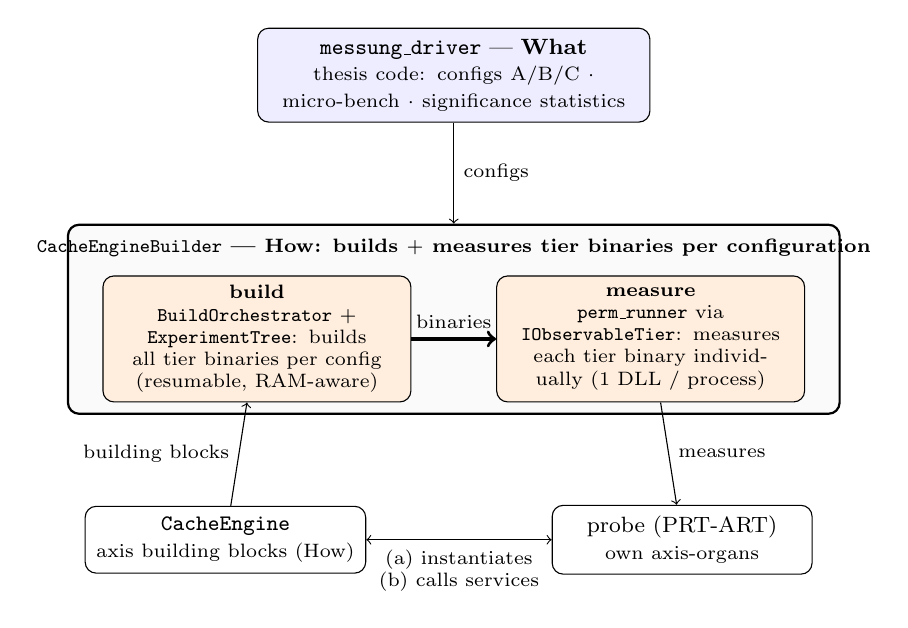
\begin{tikzpicture}[comp/.style={draw, rounded corners, align=center, font=\footnotesize, inner sep=4pt, minimum width=3.3cm},
    bm/.style={draw, rounded corners, align=center, font=\scriptsize, inner sep=3pt, text width=3.7cm, minimum height=1.6cm, fill=orange!13}]
    \node[comp,fill=blue!7,text width=4.7cm] (driver) at (0,0.6) {\texttt{messung\_driver} --- \textbf{What}\\{\scriptsize thesis code: configs A/B/C $\cdot$ micro-bench $\cdot$ significance statistics}};
    \node[draw,thick,rounded corners,minimum width=9.8cm,minimum height=2.4cm,fill=gray!4] (bbox) at (0,-2.5){};
    \node[font=\bfseries\scriptsize,anchor=north] at ([yshift=-2pt]bbox.north){\texttt{CacheEngineBuilder} --- \textbf{How}: builds $+$ measures tier binaries per configuration};
    \node[bm] (build) at (-2.5,-2.75) {\textbf{build}\\{\scriptsize \texttt{Build\-Orchestrator} $+$ \texttt{Experiment\-Tree}: builds all tier binaries per config (resumable, RAM-aware)}};
    \node[bm] (measure) at (2.5,-2.75) {\textbf{measure}\\{\scriptsize \texttt{perm\_runner} via \texttt{IObservableTier}: measures each tier binary individually (1 DLL / process)}};
    \draw[->,very thick] (build) -- node[above,font=\scriptsize]{binaries} (measure);
    \node[comp] (engine) at (-2.9,-5.3) {\texttt{CacheEngine}\\{\scriptsize axis building blocks (How)}};
    \node[comp] (probe) at (2.9,-5.3) {probe (PRT-ART)\\{\scriptsize own axis-organs}};
    \draw[->] (driver) -- node[right,font=\scriptsize]{configs} (bbox.north);
    \draw[->] (engine) -- node[left,font=\scriptsize]{building blocks} (build);
    \draw[->] (measure) -- node[right,font=\scriptsize]{measures} (probe);
    \draw[<->] (engine) -- node[below, font=\scriptsize, align=center] {(a)~instantiates\\(b)~calls services} (probe);
  \end{tikzpicture}
  \caption{The M-model focused on the build and measurement phases. The outer
  \texttt{messung\_\-driver} loop (\emph{What}, thesis code) feeds the configurations of the three
  measurement series A/B/C\@; the \texttt{CacheEngineBuilder} (\emph{How}, library) splits into the two
  genuinely interesting phases: \textbf{build} (\texttt{BuildOrchestrator}/\texttt{ExperimentTree} builds
  a standalone tier binary per configuration, resumable and RAM-aware) and \textbf{measure}
  (\texttt{perm\_runner} drives and measures each tier binary individually through the observer interface
  \texttt{IObservableTier}). The
  \texttt{CacheEngine} supplies the default axis building blocks, the probe PRT-ART its own organs;
  their bidirectional relationship ((a)~instantiates, (b)~calls services) founds the multi-probe capability. The
  \texttt{ExecutionEngine} remains the shared measurable root.}\label{fig:m-model}
\end{figure}

The builder orchestrates a \emph{three-stage evaluation}: \textbf{Stage~1} (cache-engine only) uses the
default variant per axis, \textbf{Stage~2} (probe only) replaces the overridden axes by the
probe variants and otherwise keeps the defaults, and \textbf{Stage~3} (full join, non-redundant)
combines default and all probe variants; in the code these are the merge strategies of the merge plan
--- Stage~1 is \texttt{Verbund1\_CeOnly}, Stage~2 splits into replacing (\texttt{Verbund2\_Replace}) and
hybrid mixing (\texttt{Verbund2\_Hybrid}), Stage~3 is \texttt{Verbund3\_Union} ---, which summarize the
three-stage view. Each stage can produce up to thousands of non-redundant
permutation binaries that are loaded at runtime across the C-stable module boundary as C++23 modules;
what is materialized is always a sparse, capped subset, the full product space is only
counted (Figure~\ref{fig:three-stage}).

\begin{figure}[!htbp]
  \centering
  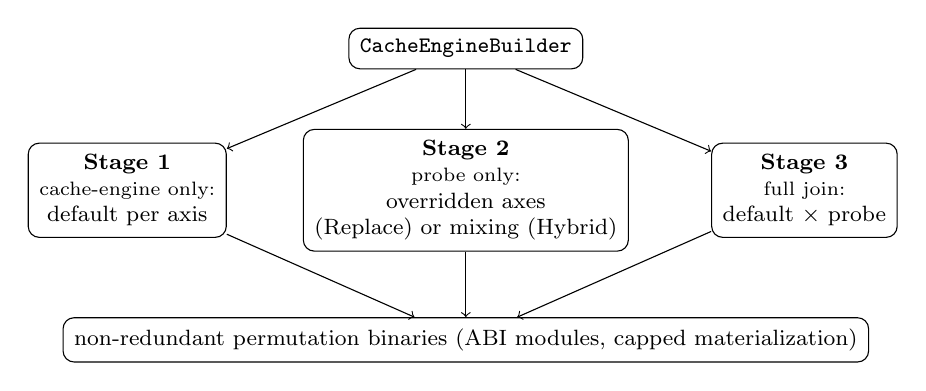
\begin{tikzpicture}[stage/.style={draw, rounded corners, align=center, font=\footnotesize, inner sep=4pt}]
    \node[draw, rounded corners, font=\footnotesize, inner sep=4pt] (b) at (0,0) {\texttt{CacheEngineBuilder}};
    \node[stage] (s1) at (-4.3,-1.8) {\textbf{Stage~1}\\\scriptsize cache-engine only:\\default per axis};
    \node[stage] (s2) at (0,-1.8) {\textbf{Stage~2}\\\scriptsize probe only:\\overridden axes\\(Replace) or mixing (Hybrid)};
    \node[stage] (s3) at (4.3,-1.8) {\textbf{Stage~3}\\\scriptsize full join:\\default $\times$ probe};
    \node[draw, rounded corners, align=center, font=\footnotesize, inner sep=4pt] (out) at (0,-3.7) {non-redundant permutation binaries (ABI modules, capped materialization)};
    \draw[->] (b) -- (s1);
    \draw[->] (b) -- (s2);
    \draw[->] (b) -- (s3);
    \draw[->] (s1) -- (out);
    \draw[->] (s2) -- (out);
    \draw[->] (s3) -- (out);
  \end{tikzpicture}
  \caption{The builder's three-stage evaluation: each stage produces non-redundant
  permutation binaries; their mapping onto the measurement series~A/B/C is shown by
  Table~\ref{tab:stage-series}.}\label{fig:three-stage}
\end{figure}

These stages do \emph{not} map one-to-one onto the three mandatory measurement series but feed them: the
default binaries of Stage~1 (including the reconstructed SOTA profiles) and the probe binaries of
Stage~2 \emph{jointly} form the comparison series~A\@; the non-redundant full join of Stage~3 is
the basis of the variation series~B\@; and the merge/regression series~C (old vs.\ new) is bound to
no single stage but runs build-spanning as an old-versus-new comparison --- over
successive states of the same configuration as well as over concrete merge points
(Table~\ref{tab:stage-series}).

\begin{table}[!htbp]
  \centering
  \caption{Mapping of the three-stage evaluation onto the mandatory measurement series}\label{tab:stage-series}
  \begin{tabular}{@{}lll@{}}
    \toprule
    \textbf{Evaluation stage} & \textbf{Content} & \textbf{feeds series} \\
    \midrule
    Stage~1 (cache-engine only) & default building blocks + SOTA profiles & A (baseline also for C) \\
    Stage~2 (probe only) & overridden axes = probe variants & A \\
    Stage~3 (full join) & default $\times$ probe, non-redundant & B \\
    build-spanning & old vs.\ new (regression and merge points) & C \\
    \bottomrule
  \end{tabular}

  \smallskip
  {\footnotesize The three evaluation stages map not one-to-one but in this assignment onto the
  three mandatory measurement series~A/B/C\@; series~C is build-/version-spanning (not bound to a single
  evaluation stage).\par}
\end{table}

The three measurement series --- all executed by the \texttt{messung\_driver} via the \texttt{ExperimentDriver} library,
configured either as three fixed series or via an external
\texttt{messreihen.xml} --- are thus: \emph{series~A} (PRT-ART vs.\ state of the art) with the modes A\_defined
(fast verification against the 8 Rank-1 full profiles) and A\_full (all 33 profiles, 30 full profiles and 3 abstract; the standard, since only the
full run delivers the bias-reduced measurement of all load profiles against all methods,
Section~\ref{sec:task-concerns}); \emph{series~B} (systematic variation of the
axis decisions under otherwise equal conditions, to isolate the contribution of each axis); and
\emph{series~C} (merge/regression old vs.\ new: concrete merge points between PRT-ART building blocks and
cache-engine permutations --- say the PRT-ART OLC with tcmalloc and ART page, the 4+1+2 pool with the
HOT page, the path prefetch with the B\textsuperscript{2}-tree page, or the MultiLevel layout with the
Wormhole page ---, run build-spanning as an old-versus-new comparison). Each series is
collected in three granularities that correspond to the three measurement levels
(Section~\ref{sec:measurement-system}).\ \emph{Micro-benchmarking} (level micro) measures each axis
over its \emph{axis interface} --- the set of functions that \emph{all} algorithms of this axis must
supply (every allocator provides memory, whichever one it is): the axis-specific
main properties, measured internally. The axis is thereby \emph{not} an interface function of the
search algorithm; its family interface functions \emph{use} the axis interfaces ---
just as axis algorithms may use foreign axis interfaces, since containers, say, are
needed everywhere.\ \emph{Macro-benchmarking} (level macro) measures the individual
\texttt{std::map} interface operations (insertion, point and range lookup, update,
deletion) against example loads, and \emph{overall benchmarking} (level wallclock, in the CacheEngineBuilder
over the load frameworks) runs the YCSB load profiles over every recombination --- w/ma/mi, in this
order. As a counter-check to the internal micro measurement, the apparatus additionally measures three
\emph{wallclock levels}: the wallclock of the axis interfaces under each algorithm, the
wallclock of the family interface functions, and the wallclock of a test load from the
load frameworks. The architectural obligation of this cut is that all axis algorithms
use exclusively axis interfaces instead of generic operating-system calls --- compiled in inline by
metaprogramming, without \texttt{std::variant} ---, so that the micro measurement of
an axis actually measures the axis. Precisely this methodology is the answer to the
separability problem: by measuring each constituent first in isolation over its axis interface
before it appears in the operation and overall context, the contributions become separately
measurable instead of remaining blended in the overall throughput.

The system reduces the space thus spanned deliberately. The golden reference catalogue --- per organ axis
two enabled representatives, the persistence axis pinned to its in-memory representative --- counts
$2^{17} = 131072$ binary identities per system permutation (per combination of the build control quantities,
Section~\ref{sec:axis-triad}), each with its full eighteen-segment path
(Section~\ref{sec:stamp-model}), and serves as the regression detector of the whole system with a
fixed CRC-64 checksum over all identities; the cardinality of the real permutation space over all
axis catalogues including their sub-axes, by contrast, is computed dynamically by the planner from its inputs
(subcommand \texttt{simulate}) --- it lies orders of magnitude above and is never a fixed
count. Three mechanisms dampen the explosion: the \texttt{<expected\_workload>} profile filter routes
only compatible workloads; the \texttt{Defined} mode runs only the declared tuples, from which
the measurement series of the manuscript are fed; and the \texttt{Full} or \texttt{Full-Sampled} mode
runs the full space or a deterministic, seed-stable 1:$n$ subset of it (default $n = 1000$).
The default workload is the full permutation over all available workloads; the routing of this
default is envisioned but not implemented (Section~\ref{sec:eval-workloads}). Full and sampled runs run on the registered
machine signatures --- prod1 (AMD Zen~5), prod2 (Intel Core i9-12900K, Alder Lake), and an
ODROID board with Intel Gracemont cores --- observing the axis compatibility reported by the platform
probe; membership of the ZIH cluster of TU Dresden is declared as a sub-axis of the
target ISA, a run there is not measured (n/a).

\section{PRT-ART as Demonstrator}\label{sec:prtart-demo}
PRT-ART is the \emph{probe} on which the load-bearing capacity of the system shows: an abstract living being that supplies some
axis-organs itself and obtains the rest via the merge strategy of the merge plan from the
default toolkit of the cache engine (Section~\ref{sec:mess-chain}) --- as monomorphic
CRTP concept axes, without runtime fallback; the hybrid
\texttt{PrtArtSearchEngine<Ts\ldots>} API remains unaffected by this, and the runtime binding occurs via
the execution-engine adapter, not via a search-engine layer of its own. The
probe repo is loaded via the plugin controller of the cache engine
(\texttt{COMDARE\_\allowbreak{}CE\_\allowbreak{}PRUEFLINGE}): its entry snippet must expressly give its
\emph{assurance} via \texttt{comdare\_\allowbreak{}pruefling\_\allowbreak{}deklarieren} ---
with the single registered capability
\texttt{pruefling\_\allowbreak{}slots\_\allowbreak{}v1}, the probe slots ---, because
presence may only refute, never permit: the deposited evidence headers can only
break the assurance, never open a gate, and a requested but non-declaring probe
breaks the configuration with an error message instead of being skipped silently; a probe-own
adapter path is deactivated and not part of this assurance.
What PRT-ART contributes lies on three levels. First, the \emph{probe slots} in its own repository:
the build axis page type, the prefetch, the value handle (ChainRef), and the telemetry tooling with the
hypothesis metrics H1/H2/H3 (in the triad a measurement-tooling sub-axis,
Section~\ref{sec:axis-triad}); the assessment of the hypothesis metrics is contained in
Chapters~\ref{ch:eval} and~\ref{ch:conclusion}. Second, the reference composition of the cache engine,
\texttt{PrtArtComposition}, which differs from the ART composition in exactly one axis --- the
path compression as redirect organ, the \emph{R} in PRT-ART\@; the optimistic lock coupling is inherited from
ART, not a PRT-ART contribution. Third, the codegen-capable probe composition, which takes sixteen of
eighteen axes from the ART composition and replaces prefetch and value handle by the
probe slots. Its further own building blocks, the 4+1+2 pool allocator
(free-list sub-axis) and the MultiLevel layout, reside in the probe repo and run in the measurement path via
the cache-engine default (attachment envisioned as a subsequent implementation step, but not
implemented); for the remaining axes it reuses existing
SOTA building blocks via the permutation configuration. Thus the probe demonstrates that the measurement system
holds: a novel living being arises from a few own organs plus the default toolkit
(Figure~\ref{fig:prtart-demo}) and is measurable over the same probe dock as every reconstructed
SOTA method.

\begin{figure}[htbp]\centering
% No \resizebox: the three-row drawing redesigned on the DE state is ~13.4cm wide (row labels plus
% legend line) and fits natively into \textwidth (16cm). Rule: resizebox only to SHRINK (cf. fig:m-model).
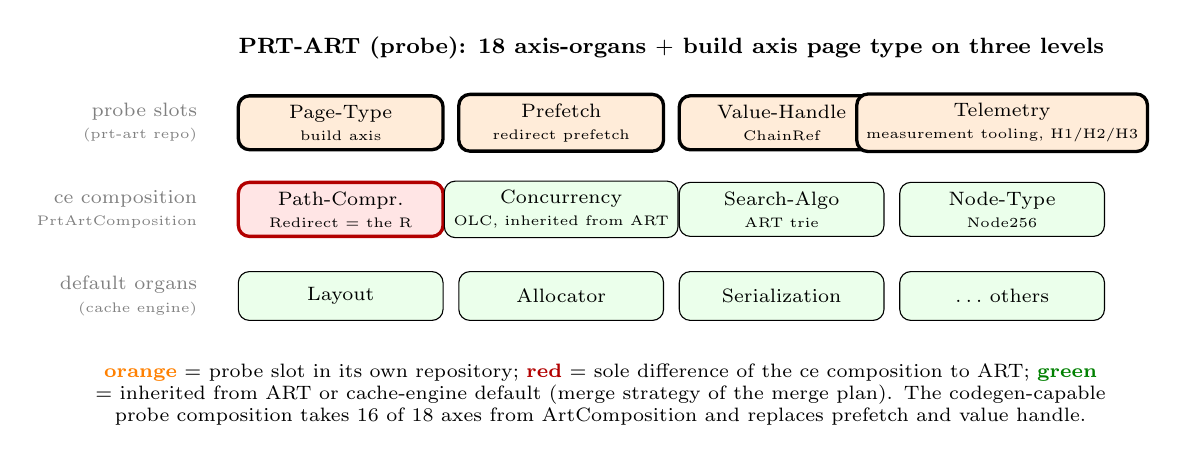
\begin{tikzpicture}[font=\footnotesize,align=center,
  prt/.style={draw,rounded corners,fill=orange!15,very thick,minimum width=2.6cm,minimum height=0.62cm,font=\scriptsize},
  ce/.style={draw,rounded corners,fill=green!8,minimum width=2.6cm,minimum height=0.62cm,font=\scriptsize},
  rd/.style={draw,rounded corners,fill=red!10,very thick,draw=red!70!black,minimum width=2.6cm,minimum height=0.62cm,font=\scriptsize},
  row/.style={font=\scriptsize,anchor=east,text=gray,align=right}]
  \node[font=\bfseries\footnotesize] at (2.9,2.55){PRT-ART (probe): 18 axis-organs $+$ build axis page type on three levels};
  \node[row] at (-3.0,1.6){probe slots\\{\tiny (prt-art repo)}};
  \node[prt] at (-1.3,1.6){Page-Type\\{\tiny build axis}};
  \node[prt] at (1.5,1.6){Prefetch\\{\tiny redirect prefetch}};
  \node[prt] at (4.3,1.6){Value-Handle\\{\tiny ChainRef}};
  \node[prt] at (7.1,1.6){Telemetry\\{\tiny measurement tooling, H1/H2/H3}};
  \node[row] at (-3.0,0.5){ce composition\\{\tiny PrtArtComposition}};
  \node[rd] at (-1.3,0.5){Path-Compr.\\{\tiny Redirect $=$ the R}};
  \node[ce] at (1.5,0.5){Concurrency\\{\tiny OLC, inherited from ART}};
  \node[ce] at (4.3,0.5){Search-Algo\\{\tiny ART trie}};
  \node[ce] at (7.1,0.5){Node-Type\\{\tiny Node256}};
  \node[row] at (-3.0,-0.6){default organs\\{\tiny (cache engine)}};
  \node[ce] at (-1.3,-0.6){Layout};
  \node[ce] at (1.5,-0.6){Allocator};
  \node[ce] at (4.3,-0.6){Serialization};
  \node[ce] at (7.1,-0.6){$\ldots$ others};
  \node[font=\scriptsize,align=center,text width=13.2cm] at (2.0,-1.85){\textcolor{orange}{\textbf{orange}} $=$ probe slot in its own repository; \textcolor{red!70!black}{\textbf{red}} $=$ sole difference of the ce composition to ART; \textcolor{green!50!black}{\textbf{green}} $=$ inherited from ART or cache-engine default (merge strategy of the merge plan). The codegen-capable probe composition takes 16 of 18 axes from ArtComposition and replaces prefetch and value handle.};
\end{tikzpicture}
\caption{PRT-ART as a demonstrator in the M-model on three levels: the four probe slots in its own repository (page type as build axis, prefetch, value handle, telemetry as measurement-tooling sub-axis, Section~\ref{sec:axis-triad}); the reference composition of the cache engine, which differs from ART in exactly one axis --- the path compression as redirect organ ---, while the optimistic lock coupling is inherited from ART\@; and the codegen-capable probe composition, which takes sixteen of eighteen axes from the ART composition and replaces prefetch and value handle. The further own building blocks (4+1+2 pool allocator, MultiLevel layout) run in the measurement path via the cache-engine default (attachment: subsequent implementation step, not implemented). Thus a complete, measurable living being arises from a few own plus many default organs.}\label{fig:prtart-demo}
\end{figure}

\section{Sharpening through Heuristics}\label{sec:heuristics}
The measurement series deliver more than rankings: from them heuristics can be won that sharpen the
measurement system step by step from a test bench into a self-optimizing delivery system.
This section develops this sharpening as a concept in three stages --- the
heuristic loop over learned load profiles, the four operating modes of the builder up to the hybrid mode
as the target picture of this thesis, and the measurement-curve type system together with the filter chain and measurement-error detection that
feed these modes with data.

\subsection{Heuristic Loop and Learned Load Profiles}\label{sec:heuristics-loop}
From the measurement series one can derive the best axis composition per load and
data-type profile and store it as a reusable profile.
\begin{figure}[htbp]\centering
\begin{tikzpicture}[font=\footnotesize,>=Stealth,thick,align=center,
  stage/.style={draw,rounded corners,fill=blue!4,minimum width=2.8cm,minimum height=1cm}]
  \node[stage] (mess) at (0,0){measurement\\{\scriptsize series A/B/C}};
  \node[stage] (profil) at (4.4,0){XML load profile\\{\scriptsize learned mapping}};
  \node[stage] (konfig) at (4.4,-2.2){configuration\\{\scriptsize best axis composition}};
  \node[stage] (filter) at (0,-2.2){workload filter\\{\scriptsize \texttt{<expected\_workload>}}};
  \draw[->] (mess)--(profil);\draw[->] (profil)--(konfig);
  \draw[->] (konfig)--(filter);\draw[->] (filter)--(mess);
\end{tikzpicture}
\caption{The heuristic loop: from the measurement series the best axis composition per load profile is learned, stored as an XML load profile, and fed back via the workload filter into the next measurement.}\label{fig:heuristic-loop}
\end{figure}

\emph{The full loop is an outlook mechanism; realized of it are the automatic selection
and the binary delivery (Section~\ref{sec:contributions}).} The selector reads the measured-value workbook ---
the xlsx workbook is the output and the standard of the apparatus; the CSV form is not a single
child document but an ordered tree of CSV files generated from the workbook with the same columns
(one overall folder per workbook, beneath it one folder per sheet, therein the CSV files of the individual
sub-axis sweeps) ---, ranks per
interface function and metric over the valid two-phase rows (median, nearest rank), determines with
competing target quantities the Pareto front of the non-dominated candidates instead of a single winner,
resolves the \texttt{binary\_id} to the binary in the store, and delivers binary, version sidecar, and manifest
as a standalone artefact. The heuristic curves arise as natural cubic splines over the
sampling points per axis and $x$-dimension; a decision lambda tree reads the break-even thresholds
from the spline intersections and chooses at a query coordinate backwards the leading binary ---
synthetic sampling points it reports as scaffolding, without valid curves it makes no decision.
Beyond mere ranking, a \emph{heuristic extraction} is envisioned as a follow-up phase after
\textbf{Persist} --- the last phase of the seven-phase pipeline (Section~\ref{sec:impl-pipeline}) ---
that automatically derives from the collected measurements which axis configuration is best per workload
and dataset. The intended mechanism is an ML classification in three steps:
first, features are extracted from the measured-value workbook per permutation --- the load-profile and dataset features (workload type,
key distribution, write/read share, alphabet and prefix characteristics, as well as key and
value data type) and the axis assignment ---, with the
best performance measured per load pattern (say throughput or tail latency) as the target quantity; over these an \emph{ML classifier} learns the mapping
from load-profile/axis features to the best configuration; and it delivers per workload/dataset class
the recommended axis composition without re-running the entire permutation space. The result is
persisted as a reusable \emph{XML load profile} --- symmetric to the measurement-series XML configurations
--- and can be fed back into the \texttt{<expected\_workload>} filter without a full re-measurement;
this closes the loop between measurement, learned heuristic, and configuration-guiding selection
(Figure~\ref{fig:heuristic-loop}). This \emph{measure $\to$ profile $\to$ config $\to$
filter} loop is the classical, established form of \emph{empirical, measurement-driven autotuning}:
it stands in the line of autotuning frameworks such as OpenTuner~\cite{ansel2014opentuner} and the
measure-in-the-loop autotuners FFTW~\cite{frigo1998fftw} and ATLAS~\cite{whaley2001atlas}; the
load-profile-driven configuration choice with workload filter finds its database counterpart in
OtterTune~\cite{vanaken2017ottertune} and in the Database Tuning Advisor with workload compression~\cite{agrawal2005autoadmin},
the online runtime-near variant in Active Harmony~\cite{tapus2002activeharmony}; the term
\enquote{software-in-the-loop} itself originates from the X-in-the-loop validation taxonomy~\cite{tibba2016xil}.
The ML classification is not implemented and remains reserved for future work
(Chapter~\ref{ch:conclusion}); the loop itself, however, is only the first stage of a larger
operating target picture, which the following subsection develops.

\subsection{The Four Operating Modes of the Builder}\label{sec:heuristics-modes}
The heuristic loop is the core of an operating regime of \emph{four} operating modes of the builder
interface that build on one another. From the run chain build $\to$ measure $\to$ compare $\to$ release
(Section~\ref{sec:anatomy-levels}, Figure~\ref{fig:modi-kette}) these operating target pictures are to be
distinguished, in which the apparatus is operated; the assignment is unambiguous: the \emph{measurement mode}
comprises build and measure, the \emph{evaluation mode} is compare, the \emph{working mode} is the
release of a single binary, and the \emph{hybrid mode} is the release of a hybrid recombination,
whose chain repeats on the hybrid level. The first mode is the operation of the apparatus; modes
two through four are the declared goal of this thesis and are recorded here as a concept. The
hybrid mode is thereby an extended, optional construct: the core of the thesis is the measuring through
and generating of the tier binaries together with break-even analysis before every application of the hybrid, and the thesis
does not go in the chain beyond the comparison stage of the hybrid level (\texttt{hybrid-compare}) after the
delivery stage of the single binary (\texttt{single-release}). To be distinguished from these four
operating modes is the \emph{paper isolation mode} asked for in sub-question RQ2.c (Section~\ref{sec:rqs}):
an operating mode that offers the design constituents of exactly one
publication as an \emph{axis set} --- the closed axis set of this one reference design,
with measurement and system axes still free-standing --- in isolation, in order to measure the publication
faithfully; it is not implemented and remains outlook (Section~\ref{sec:outlook}).

In the \emph{measurement mode} --- the operation that Section~\ref{sec:measurement-system} describes --- the
builder runs the measurement series over the admitted permutations. After completion of the measurement the
framework knows the properties of all admitted axis algorithms against the recombination of all
admitted load-profile frameworks and workloads. The \emph{evaluation mode} condenses these
measurements: from them emerge minimal strands of the permutations of all properties against one another
for certain \emph{workload clusters} --- for groups of similar loads, the small set of
axis compositions that dominates them remains. For this, workloads are clustered according to sequences,
as similar as possible, of equal access patterns on the family and genus interfaces of the tier binaries: every
load framework runs through its planned strategy once dry, and sequence, frequency, and
requirements of its interface calls are noted --- what a run of the framework statically
gives of itself. From this arises per profile a directed transition graph of the interface accesses with
absolute and relative successor probabilities (the mapping of an interface onto itself is
admitted as an edge); its edge matrix is evaluated with the EM algorithm~\cite{dempster1977em},
and the distances of the centres of the probability point clouds from one another yield
per profile a \emph{point-cloud word} of variable length (shorter when interfaces are not called
--- null-filtered). The lexicographic sorting of these words is the measurement order:
adjacent words are similar loads and are --- no matter from which framework they
stem --- run one after another. This procedure is not implemented in the code; it is at the same time the
fourth evaluation component of the hybrid tier (Section~\ref{sec:heuristics-curves}).

The \emph{working mode} is the production goal: the builder interface keeps all tier binaries relevant for the currently
stochastically frequent workload load and interface function preloaded in
main memory and internally switches the tier binary with its specifically optimal
axis permutations at the ABI-stable interface --- the same binary-switching mechanism that the
measurement mode uses, only load-driven instead of measurement-driven. In this, the
compile-time principle remains preserved at the correct level: there is no runtime switch \emph{inside} the tier --- the binaries
themselves remain compile-time-permuted; switching happens \emph{between} preloaded binaries at
the deliberate ABI boundary. The probe dock of the family (Section~\ref{sec:anatomy-levels}) is called in this
mode the \emph{working dock}: the same interface through which the measurement mode tests now delivers the
productive answers. The dock layer of this switch is implemented --- the dock contracts, the probe dock,
the dock factory as the sole construction site, the dock field with attachment and detachment, the parser
of the hybrid section of the XML, and the binary proxy, which makes a hybrid binary outwardly an ordinary
tier binary ---; router, eviction, and the \texttt{.so} export of the switch are not implemented.
The hybrid always compiles with the help of the CacheEngineBuilder, never by itself.

On switching from one tier binary to another, every participating tier binary must contain a further
\emph{state surface} compiled in, which reads and re-sets the state in the hybrid mode ---
sparse: every binary keeps its state and pulls in only the versioned changed blocks, a
checkpoint procedure after the \emph{Memento} pattern~\cite{gamma1994patterns}, which bypasses the interfaces
and tracks the memory block-wise only for changed regions. Main memory multiplies
thereby, because all participating binaries hold the total state, of which always one is in front and current.
The state surface is a compiled-in, metaprogrammed sidecar library that occurs only in the
hybrid pattern --- in single operation a tier binary does not contain it; therefore two
release artefacts are stored, a release for single operation without sidecar and a release for the
hybrid operation with sidecar (Section~\ref{sec:lager}). The hybrid binary organizes the states in the
protocol of the switch and enforces the checkpointing for all metaprogrammatically attached tier binaries:
the computed switch per hybrid request generates a memory reconciliation between the
tier binaries and then passes the request through to the chosen tier binary. State surface and sidecar
are not implemented.

The \emph{hybrid mode}, finally --- the goal of this thesis --- combines working mode and measurement. Its
centrepiece is that the heuristic adapter is a \emph{family} of its own with its own genus --- the fourth
family \texttt{HeuristikAdapter} with the reroute genus \texttt{FunctionInterfaceReroute}
(Section~\ref{sec:anatomy-levels}): it adopts by metaprogramming the family and
genus interfaces of its tier binaries, is itself compiled into a tier binary, and docks at the
probe dock of the builder like every single tier; it passes commands via the
\emph{Command} pattern~\cite{gamma1994patterns} on to the single tier binaries statically assigned to it.
To the outside it is indistinguishable from a single binary, because its binary exports the same
mandatory symbols as every other and reports as genus the inherited target genus --- classification
(the kind of the reroute) and pass-through lie on separate levels. The recombination of the
heuristic tier binaries to be used is thereby itself permutable against the existing single
tier binaries; the heuristic adapter can therefore use the measurement function curves for estimates and
compile an optimal multidimensional recombination that is unambiguously usable as a search-algorithm hull
through its ABI-stable family interface --- to the outside a \emph{virtual whole
tier binary}. At the same time the hybrid mode measures along: over the optimized
recombination the combined wall-clock time as well as macro- and micro-benchmarks are logged per measurement command
across all tier binaries and operations.

Thereby the hybrid mode delivers the \emph{heuristic counter-proof}: after entry into the working mode the
heuristic tier binary is measured anew --- its wall-clock behaviour in comparison against the best
single binaries and against the reconstructed paper algorithms decides whether the heuristic
recombination reaches the performance predicted by the curves. The curves that the counter-proof checks are the
spline curves per axis and $x$-dimension with their break-even intersections
(Section~\ref{sec:heuristics-loop}); in the stage compare it is computed from the measurement store which
tier binary or hybrid recombination must, according to the measurement, be the best, and in the stage release
the maximally optimized compiled binary without compiled-in measurement sensors is measured through once more ---
whether its wall clock without measurement insight even undercuts the previously measured total time. The
comparison against the reconstructed paper algorithms presupposes per publication a wall-clock reference,
which is missing as a data source and is to be determined per method from the respective publication; the paper comparison
takes precedence over the Pareto selection. The goal of the thesis is thus formulated twice over: to determine the
best recombination or the best single binary against all axis properties ---
especially cache-line awareness --- and in the end to provide both in production-ready form,
the best single binary \emph{and} the heuristic tier binary consisting of the best mixed cache-aware binaries for the measured loads. All four modes shall
thereby be documented automatically via the evaluation chain of the definition layer (Section~\ref{sec:anatomy-layers});
the measured-value tables and diagrams of this thesis itself are the product
of the compare stage of this chain, and the assessment of the counter-proof is defined by Chapter~\ref{ch:eval}.
\subsection{Measurement-Curve Type System, Filter Chain, and Measurement-Error Detection}\label{sec:heuristics-curves}
For the evaluation and the hybrid mode to hold, the evaluation needs more than flat
result tables. As a target picture this thesis formulates a \emph{measurement-curve type system} for this; implemented of
it is a first approach --- a curve fit over one axis and one $x$-dimension as a natural cubic
spline (Section~\ref{sec:heuristics-loop}) ---, while the type-system key framework $\times$
workload $\times$ operation $\times$ size is not implemented. Every tier-binary total permutation receives
per measurement axis a wall-clock measurement curve over the working set --- say the lookup latency as a function of the
fill size ---, separated by load-profile framework, workload type, working-set size,
operation type, and observer type and per measurement level wallclock, macro, and micro
(Section~\ref{sec:measurement-system}); every axis is swept separately in the experiment tree compile-statically as well as
runtime-dynamically, so that every axis receives a complete overview of its
properties and individual measurements. Taken together over all permutations there thus arises per
tier binary a multidimensional measurement database, from which the heuristic curves of the loop
(Section~\ref{sec:heuristics-loop}) are read; the synthesized curves are kept as files in the
store (Section~\ref{sec:lager}). The cardinality of every dimension of this
type system is to be organized strategically into classes and hierarchies: design-fixed constants (say the
eighteen organ axes), registered, dynamically growing quantities (the measurement categories,
Section~\ref{sec:axis-triad}), profile-bound products (what an experiment profile admits as assignments),
and runtime-free iteration spaces (the dynamic sampling points per static binary) --- thus
the system axes remain able to support the evaluation across all levels.

The compare stage is composed of five evaluation components that are gradations of a chain,
not alternatives: first, the ranking per metric with Pareto front and delivery (implemented,
Section~\ref{sec:heuristics-loop}); second, the spline curves with the break-even decision (implemented as a
first approach); third, the filter chain over the permutation families (mechanism implemented,
evaluation links not implemented, next paragraph); fourth, the live ranking of the preloaded tier binaries in the
hybrid tier from the interface accesses recorded at runtime and their
transition probabilities --- the same clustering procedure as for the measurement order
(Section~\ref{sec:heuristics-modes}), which holds the known interface suitabilities of a tier binary against the
measured requirements and passes the request through to the best binary (not implemented); and
fifth, the measurement-error interpolation over the measurement constellations (not implemented, paragraph after next).

From the evaluations there emerges a \emph{filter chain}: every chain link checks, based on the curves so far,
whether a permutation family is pursued further, and otherwise passes the decision on to the
next link --- the design pattern \emph{Chain of Responsibility}~\cite{gamma1994patterns}. The
chain is located in the CacheEngineBuilder, because it controls the \emph{generation} of the next build round
and closes the feedback edge from the selection to the provisioning: evaluation, filter, then
the decision which permutations are built next and which are discarded. Since in compare
build and measure have already been run through, it at the same time filters from the measured values for the release
which binary is statistically the fastest for a purpose according to the properties demanded in the XML
--- the default is the execution time, further filters are not the subject of this
thesis. Implemented are the mechanism (with the verdicts Pass, Reject, and pass-on: a
candidate survives exactly when no link rejects it) and a core link for the resumption of
interrupted runs; the evaluation links --- the paper comparison, which lacks the reference source, and
the Pareto dominance, which lacks the type-system key --- follow as further links, with the precedence
of the paper comparison over the Pareto selection.

Finally, the hybrid mode needs a control of the measurement error that the measurement instances themselves
introduce --- observers cost time. The three measurement facilities --- the wall clock in the
CacheEngineBuilder, the genus interface time of the tier binary (macro), and the axis interface time
(micro) --- can be built as a three-phase contract construction between CEB and tier binary in all
arrangements: with three facilities $3! = 6$ probe-dock constellations, which only need to be measured at the tier binary,
with an interposed hybrid tier binary $4! = 24$ constellations of the chain
CEB--hybrid--tier; over several hybrid stages connected in series (hybrid meta-meta stages,
compile-statically extensible via the XML) the number is dynamically $n \times m$ and is never presented
statically. From the differences of all measured values with built-in measurement sensors against the respectively most accurate
remaining total time, related to the number of the finest interface accesses, a
mathematical procedure interpolates the measurement error over the constellation matrix and computes it out of the
published results --- the fifth evaluation component. The three previously named
build variants of the same experiment --- first, observers in all tier binaries \emph{and} in the
heuristic hybrid tier, second, observers only in the heuristic tier binary, third, observers in none,
only the wall clock --- are three of these constellations. Complementarily follows a \emph{fourth step}
of the final heuristic assembly: the tier binaries subordinate to the heuristic tier (not the
finally optimized main binary) are rebuilt without micro- and macro-benchmarks and without observers and
compared purely on the wall clock against all known tier-binary permutations and against the known
paper algorithms --- with the paper comparison taking precedence. The validity criterion of every
constellation is that the measurement with measurement sensors is slower than the same without. What is laid is the
foundation: the measurement gates per compiled artefact as a fingerprint member, whose coverage CEB off, tier on is proven by a test,
and the declared non-observation per measured value (Section~\ref{sec:axis-triad}); the
interpolation and the constellation matrix are not implemented.

This keeps clearly apart what is implemented and what is a goal. Implemented are the measurement apparatus with its
merge stages, the evaluation chain up to tables and diagrams, the curve fit as a first approach together with
break-even tree, the Pareto selection with delivery, the filter-chain mechanism with resumption link,
the dock and classification layer of the hybrid tier together with XML parser and binary proxy, and the
measurement gates per compiled artefact.
The measurement runs of the complete measurement series are not available. Not implemented are the evaluation links of the
filter chain, router, eviction, and \texttt{.so} export of the hybrid switch, the state synchronization with sidecar,
the workload clustering, the measurement-error interpolation, the type-system key of the measurement curves, the
collection per axis-interface parameter set, and the attachment of the P-/E-core measurement to the run profile. The
assessment of the heuristic counter-proof is taken up by Chapter~\ref{ch:eval}; the placement of the outlook
beyond this thesis is given by Chapter~\ref{ch:conclusion}. First, Chapter~\ref{ch:impl} deepens the
concrete implementation of the building blocks introduced here.
